\documentclass[]{politex}
% ========== Opções ==========
% pnumromarab - Numeração de páginas usando algarismos romanos na parte pré-textual e arábicos na parte textual
% abnttoc - Forçar paginação no sumário conforme ABNT (inclui "p." na frente das páginas)
% normalnum - Numeração contínua de figuras e tabelas 
%	(caso contrário, a numeração é reiniciada a cada capítulo)
% draftprint - Ajusta as margens para impressão de rascunhos
%	(reduz a margem interna)
% twosideprint - Ajusta as margens para impressão frente e verso
% capsec - Forçar letras maiúsculas no título das seções
% espacosimples - Documento usando espaçamento simples
% espacoduplo - Documento usando espaçamento duplo
%	(o padrão é usar espaçamento 1.5)
% times - Tenta usar a fonte Times New Roman para o corpo do texto
% noindentfirst - Não indenta o primeiro parágrafo dos capítulos/seções


% ========== Packages ==========
\usepackage[utf8]{inputenc}
\usepackage{amsmath,amsthm,amsfonts,amssymb}
\usepackage{graphicx,cite,enumerate}


% ========== Language options ==========
\usepackage[brazil]{babel}
%\usepackage[english]{babel}


% ========== ABNT (requer ABNTeX 2) ==========
%	http://www.ctan.org/tex-archive/macros/latex/contrib/abntex2
%\usepackage[num]{abntex2cite}

% Forçar o abntex2 a usar [ ] nas referências ao invés de ( )
%\citebrackets{[}{]}


% ========== Lorem ipsum ==========
\usepackage{blindtext}



% ========== Opções do documento ==========
% Título
\titulo{Sistema de Monitoramento e Controle da Fermentação de Cervejas}

% Autor
\autor{José Henrique Camargo Leopoldo e Silva\\
       Rafael Jardim Pastor}

% Para múltiplos autores (TCC)
%\autor{Nome Sobrenome\\%
%		Nome Sobrenome\\%
%		Nome Sobrenome}

% Orientador / Coorientador
\orientador{Prof. Dr. Carlos Eduardo Cugnasca}
% \coorientador{Nome do coorientador (opcional)}

% Tipo de documento
\tcc{Eletricista}
%\dissertacao{Engenharia Elétrica}
%\teseDOC{Engenharia Elétrica}
%\teseLD
%\memorialLD

% Departamento e área de concentração
\departamento{Nome do departamento}
\areaConcentracao{Engenharia Elétrica}

% Local
\local{São Paulo}

% Ano
\data{2020}




\begin{document}
% ========== Capa e folhas de rosto ==========
\capa
\falsafolhaderosto
\folhaderosto


% ========== Folha de assinaturas (opcional) ==========
%\begin{folhadeaprovacao}
%	\assinatura{Prof.\ X}
%	\assinatura{Prof.\ Y}
%	\assinatura{Prof.\ Z}
%\end{folhadeaprovacao}


% ========== Ficha catalográfica ==========
% Fazer solicitação no site:
%	http://www.poli.usp.br/en/bibliotecas/servicos/catalogacao-na-publicacao.html


% ========== Dedicatória (opcional) ==========
\dedicatoria{Dedicatória}


% ========== Agradecimentos ==========
\begin{agradecimentos}

Thanks...

\end{agradecimentos}


% ========== Epígrafe (opcional) ==========
\epigrafe{%
	\emph{``Epígrafe''}
	\begin{flushright}
		-{}- Autor
	\end{flushright}
}


% ========== Resumo ==========
\begin{resumo}
Resumo...
%
\\[3\baselineskip]
%
\textbf{Palavras-Chave} -- Palavra, Palavra, Palavra, Palavra, Palavra.
\end{resumo}


% ========== Abstract ==========
\begin{abstract}
Abstract...
%
\\[3\baselineskip]
%
\textbf{Keywords} -- Word, Word, Word, Word, Word.
\end{abstract}


% ========== Listas (opcional) ==========
\listadefiguras
\listadetabelas

% ========== Listas definidas pelo usuário (opcional) ==========
\begin{pretextualsection}{Lista de símbolos}

Lista de símbolos...

\end{pretextualsection}

% ========== Sumário ==========
\sumario



% ========== Elementos textuais ==========

% \part{Introdução}
	
% \chapter{Capítulo com epígrafe}
% \capepigrafe[0.5\textwidth]{``Frase espirituosa de um autor famoso''}{Autor famoso}

% \blindtext

% \begin{citacaoLonga}
% 	\blindtext
% \end{citacaoLonga}

% \blindtext



% \blinddocument

\chapter{Introdução}

\section{Objetivo}

O objetivo geral deste estudo é desenvolver um protótipo de um sistema que realize o monitoramento e controle do processo de fermentação de cervejas.
O objetivo específico é possibilitar às cervejarias de pequeno e médio porte o desenvolvimento da capacidade de testes de novas receitas de cervejas, 
a fim de garantir a reprodutibilidade e qualidade das mesmas por meio do controle do processo de fermentação.

\section{Resumo}
Na produção de cervejas, a fermentação é um complexo processo bioquímico cuja função primária é converter os açúcares obtidos dos grãos maltados em etanol, tendo grande impacto no sabor, aroma, aparência e textura do produto. 
As principais variáveis da fermentação são a densidade do líquido em fermentação, que indica a evolução do processo, e a temperatura do líquido, que impacta diretamente no funcionamento da levedura de modo que um controle preciso evitar subprodutos indesejados e contaminações que impactam significativamente qualidade final do produto. 
O objetivo geral desse projeto é criar um protótipo de um sistema que realize o monitoramento dessas variáveis no processo e controle de temperatura, de modo a garantir resultados mais precisos e reprodutíveis, voltado para cervejarias de pequeno e médio porte que realizem testes de novas receitas e necessitem de alto grau de controle para escalas pequenas de produção. 
O sistema idealizado é composto por dois principais subsistemas: (i) um físico, agregando o controlador, hardware com sensores e atuadores e software embarcado; e (ii) um digital, que capta, processa e disponibiliza todas as informações adquiridas para o usuário. A execução do projeto será guiada por várias iterações curtas e prototipagem, focando na resolução de algumas milestones a cada iteração, com a finalidade de acelerar a obtenção de resultados.
Deste modo, para a aquisição de conhecimento técnico e de negócio necessários para a execução do projeto será feito um levantamento e estudo de material bibliográfico adequado, entrevistas com mestres-cervejeiros para o qual o produto se destinaria e análise de soluções já existentes no mercado, dentro e fora do país.

\section{Organização do Trabalho}


\chapter{Contexto}

Esse projeto tem natureza multidisciplinar, buscando harmonizar a bioquímica do
processo de produção de cervejas com sistemas de controle e automação e
geração e análise de dados estudados na Engenharia Elétrica. Em sua primeira
parte, será estudado o funcionamento das leveduras e como o ambiente age sobre
seu processo metabólico, enquanto na outra parte, são estudados sensores,
atuadores e arquitetura de Internet das Coisas para captação, processamento e
disponibilização de informações referente a ação dos microrganismos.

\section{História da Cerveja}

% // TODO: Colocar fontes bibliográficas

A cerveja pode ser considerada a bebida alcoólica mais antiga do mundo, e atualmente tem uma importância social e econômica muito grande. Durante anos, a sua produção ganhou diversas mudanças, melhorias e adaptações até chegar nas variedades de forma e sabor conhecidas atualmente. 


A cerveja provavelmente teve origem na revolução agrícola, na qual os humanos começaram a abandonar o nomadismo e se estabeleceram em comunidades que cultivam diversos grãos. Com o armazenamento de cereais, é provável que essa origem tenha sido acidental, com uma fermentação espontânea da cevada. Os mais antigos registros dessa bebida podem ser encontrados na antiga região mesopotâmia, atual Irã, e são datados em 2800 a.C. A sua importância em comunidades antigas do oriente médio era tanta, que em 1760 a.C., foi criada a primeira lei que regulamenta a produção e venda de cerveja. A lei conhecida como Estela de Hamurabi regulamentou a comercialização, fabricação e consumo, estabelecendo uma ração diária de cerveja para os habitantes da região. 


Como o consumo da cerveja era mais seguro do que a água, visto que o processo de fervura ajuda a purificar a bebida. O  seu consumo em algumas sociedades era visto como uma necessidade básica diária. Esse fato ajudou a aumentar a popularidade da bebida na Europa durante a idade média, principalmente nas comunidades Germânicas. Uma das instituições mais importantes para o desenvolvimento dos processos de produção eram os mosteiros dessa região e época. Os monges eram responsáveis pela fabricação da bebida e como eram os únicos que reproduziam os manuscritos, puderam conservar e aperfeiçoar a sua produção, sendo muito influentes até hoje. Eles foram responsáveis por incluir diversas ervas na fabricação, sendo a mais importante delas o lúpulo, utilizado para trazer o amargor da bebida. 


Uma das leis mais conhecidas e importantes da indústria cervejeira é a da pureza Alemã. Devido a diversas mudanças aplicadas pelos fabricantes e a percepção de uma queda de qualidade, essa lei foi criada no século XIV na região da Bavária (Sul da Alemanha) buscando uma padronização da bebida. A lei instituiu que a cerveja deveria ser fabricada apenas com os seguintes ingredientes: água, malte de cevada e lúpulo. Atualmente, apesar da legalização do uso de qualquer ingrediente na região, muitos cervejeiros ainda seguem essa restrição e ela é um sinônimo de qualidade. 


Uma das mais importantes inovações na fabricação foi a Pasteurização, que permite a preservação do gosto por mais tempo. O processo consiste, basicamente, no aquecimento da bebida a uma determinada temperatura, por determinado tempo, e depois a bebida é resfriada de forma a eliminar os microorganismos ali presentes. O processo foi nomeado pelo seu criador o francês Louis Pasteur que atendendo a solicitação de alguns dos vinicultores e cervejeiros da região que lhe pediram para descobrir como os vinhos e a cervejas azedaram. Durante sua investigação, através do uso de microscópio, ele pôde constatar que a levedura ocasionava este processo e assim criou esse processo de purificação. A partir dele, a indústria cervejeira conseguiu chegar em um novo nível e crescer em escala e alcance, sendo essencial para grandes fábricas atualmente. 


Atualmente, a indústria de cerveja movimenta milhões de dólares anualmente e uma das divisões que mais cresce são as microcervejarias. No Brasil começaram esses pequenos produtores começaram a surgir na década de 90. Em 2012 as cervejas especiais representavam 8\% do mercado nacional da bebida em 2012 e encerraram 2014 com uma participação de 11\%, segundo o Sindicato Nacional da Indústria da Cerveja, que aponta a existência de 300 microcervejarias no País. A projeção é de que essa cota suba para 20\% em 2020.


\section{Fabricação de Cervejas}

\citeonline{Lewis} apresenta a produção de cerveja como uma atividade que deve equilibrar 
séculos de tradição e arte, desenvolvida por gerações de cervejeiros, e a abordagem científica 
e avanços tecnológicos, de forma que estes possam proporcionar maior entendimento, controle e melhorias 
sobre o processo mas sem abandonar suar raízes históricas e descaracterizá-lo. 
Justamente, as etapas principais do processo ainda seguem a produção tradicional, apesar
da evolução de métodos e técnicas adicionais.

Nesta seção é descrito o processo mais comum de produção de cervejas, considerando os principais
ingredientes: água, malte, lúpulo e levedura. Tradicionalmente, são utilizados grãos maltados de cevada,
mas atualmente podem ser utilizados outros grãos, maltados ou não, como por exemplo: trigo, milho, arroz e aveia.
A partir da descrição de \citeonline{Kunze}, são listadas as principais etapas de produção:


\begin{enumerate}
    \item Maltagem dos grãos: processo de germinação parcial e controlada dos grãos, com a finalidade
de produzir enzimas como a amilase. A germinação é interrompida por um processo de secagem quando atinge o estágio desejado.
A partir desse momento, os grãos passam a ser denominados malte;
    \item Moagem do malte: quebra do malte em pequenos fragmentos para expor as enzimas e componentes internos. É desejável
que parte da casca seja mantida intacta para auxiliar na filtragem após a mostura;
    \item Mostura: o malte moído é misturado em água, e aquecida em temperaturas
que estimulem a ação das enzimas obtidas na maltagem. As enzimas
realizam a quebra de moléculas insolúveis de amido em moléculas menores
de açúcares, que são dissolvidas, formando uma solução denominada mosto;
    \item \textit{Lautering}: o mosto é separado do restante do malte que não foi dissolvido. As
cascas dos grãos auxiliam essa etapa formando um filtro natural, mas também podem ser utilizados filtros;
    \item Fervura: o mosto é fervido, consequentemente: a ação enzimática é
interrompida e a solução é esterilizada. Nessa etapa, lúpulos são adicionados em diferentes
momentos da fervura, fornecendo extratos que conferem amargor e aroma à cerveja;
    \item Fermentação: após o resfriamento do mosto, leveduras são adicionadas e a solução é aerada. 
Os açúcares são consumidos pelo metabolismo das leveduras, gerando etanol e dióxido de carbono;
    \item Maturação: após o consumo dos açúcares, as leveduras passam a reabsorver parte dos
subprodutos gerados durante a fermentação, melhorando a qualidade geral da bebida. Ao final do processo, as leveduras floculam e decantam, podendo ser extraídas e reaproveitadas;
    \item Envase: transferência para o recipiente final. Nessa etapa, também é
realizada a carbonatação da bebida, geralmente por injeção de gás carbônico
ou por meio de uma segunda fermentação, aproveitando-se leveduras ainda presentes na solução.
Industrialmente, é comum a filtragem pré-envase, e a pasteurização pós-
envase.
\end{enumerate}

\subsection{Fermentação e Maturação}

% // TODO: Melhorar Fermentação e Maturação

\citeonline{Kunze} posiciona a fermentação como o processo mais importante da produção de cervejas, sendo as etapas
antecedentes responsáveis para garantir as condições necessárias para que as leveduras possam converter os açúcares,
extraídos do malte e quebrados em moléculas menores pelas enzimas, em álcool e gás carbônico. As leveduras consomem 
os açúcares para gerar energia e se reproduzirem, e nesse processo também geram centenas de subprodutos como ésteres, álcoois pesados e compostos sulfúricos que mesmo em pequena quantidade são essenciais para as características organolépticas da cerveja, como
pontuam \citeonline{YeastWhite}.

Leveduras são organismos unicelulares membros do reino fungi. Na produção de cervejas são utilizadas principalmente 
duas espécies: a \textit{Saccharomyces cerevisie} (em cervejas do tipo \textit{Ale}) e a \textit{Saccharomyces pastorianus} (em cervejas do tipo \textit{Lager}). Ao serem inoculadas ao mosto, as leveduras rapidamente absorvem o oxigênio dissolvido para revitalizar sua membrana celular e iniciar a absorção dos açúcares e nutrientes do mosto. 

A partir do açúcar absorvido, a levedura pode convertê-lo em energia por meio da respiração aeróbica que ocorre na presença de oxigênio, ou pela respiração anaeróbica que ocorre na ausência de oxigênio ou em solução com alta concentração de glicose (pelo chamado efeito de Crabtree). 
Além da produção energia no formato de moléculas de adenosina trifosfato (ATP), a respiração anaeróbica também produz etanol e gás carbônico, por isso também é denominada de fermentação alcoólica; a equação \ref{eq:fermentacao} ilustra essa reação. A molécula de ATP provém energia para a síntese de proteínas e replicação de DNA, necessários para a multiplicação celular.

\begin{equation}
    Glicose + 2 ADP + 2 Fosfato \longrightarrow 2 Etanol + 2 CO_2 + 2 ATP
    \label{eq:fermentacao}
\end{equation}

A etapa de fermentação e maturação de uma cerveja leva em média entre 7 e 14 dias, desde a inoculação das leveduras até a cerveja estar pronta para envase. Vale notar que podem ser aplicados processos extras na maturação que prolonguem esse tempo.
Para uma fermentação básica, \citeonline{YeastWhite} classificam o processo em 3 fases, que ocorrem com certo grau de sobreposição:
\begin{enumerate}
    \item Fase de retardamento, durante as primeiras quatro a 15 horas após a adição
da levedura no mosto, caracterizada pela climatização das células ao
ambiente e preparação para a próxima fase;
    \item Fase de crescimento exponencial, que dura entre quatro horas e quatro dias,
quando ocorre o consumo dos açúcares e replicação logarítmica das células
de leveduras;
    \item Fase estacionária, em que o crescimento diminui e alguns compostos, como o diacetil, são
absorvidos pelas leveduras, maturando o produto durante três a dez dias.
\end{enumerate}

A variação nas durações das etapas é decorrente tanto da quantidade e saúde das leveduras inoculadas, quanto da temperatura 
durante a fermentação. Tradicionalmente, cervejas do tipo \textit{Ale} são fermentadas a 20°C e cervejas do tipo 
\textit{Lager} a 10°C. Temperaturas inferiores tornam o processo mais lento, e em casos extremos culminar na parada do processo, impedindo a fermentação completa ou que os subprodutos como o diacetil seja absorvido pelas leveduras. temperaturas superiores aceleram a atividade celular, tornando o processo mais rápido, mas também podendo fazer com que as leveduras se multipliquem demais e gerem uma quantidade de subprodutos alta que pode impactar negativamente na qualidade da bebida, gerando sabores indesejados denominados \textit{off-flavors}.

Justamente por essa razão, o controle de temperatura durante a fermentação é essencial para a obtenção de um produto de 
qualidade com resultados consistentes, principalmente nas primeiras 72 horas do processo, que representam o pico de multiplicação celular, geração de calor decorrente da atividade celular e produção de sub-produtos.

Após a temperatura, a segunda variável mais importante para se monitorar é a densidade relativa do mosto 
(\textit{specific gravity} em inglês) que indica o grau de evolução do processo. Como parte do gás carbônico produzido 
na equação \ref{eq:fermentacao} é dissolvido e capturado pela atmosfera, a densidade do mosto diminui durante a fermentação à
medida em que os açúcares vão sendo consumidos. A partir disso, é possível: identificar as etapas da fermentação pelo
gráfico de evolução da densidade relativa ao longo do tempo; estimar a graduação alcoólica a partir dos valores inicial e 
final da densidade relativa; e estipular o grau de atenuação, ou quanto dos açúcares foram consumidos pelas leveduras.

Uma terceira variável relevante durante a fermentação é o pH, que sofre uma leve queda durante o processo, e pode ser 
utilizado principalmente como uma amostra das condições iniciais da fermentação, com intuito de se obter reprodutividade do 
processo, e também pode servir como uma variável de diagnóstico de problemas que podem ocorrer como não adaptação das 
leveduras ao mosto e contaminação.

Com caráter ilustrativo, é incluído gráfico com o perfil dessas e outras variáveis durante a fermentação de uma cerveja 
do tipo \textit{Lager} (Figura \ref{fig:variaveis_fermentacao}). Na figura, \textit{specific gravity} se refere à
densidade relativa do mosto, e \textit{cells in suspension} à quantidade de células de levedura em suspensão, vale notar que 
ao final do processo, as leveduras floculam e decatam, por isso a queda.

\begin{figure}[H]
    \centering
    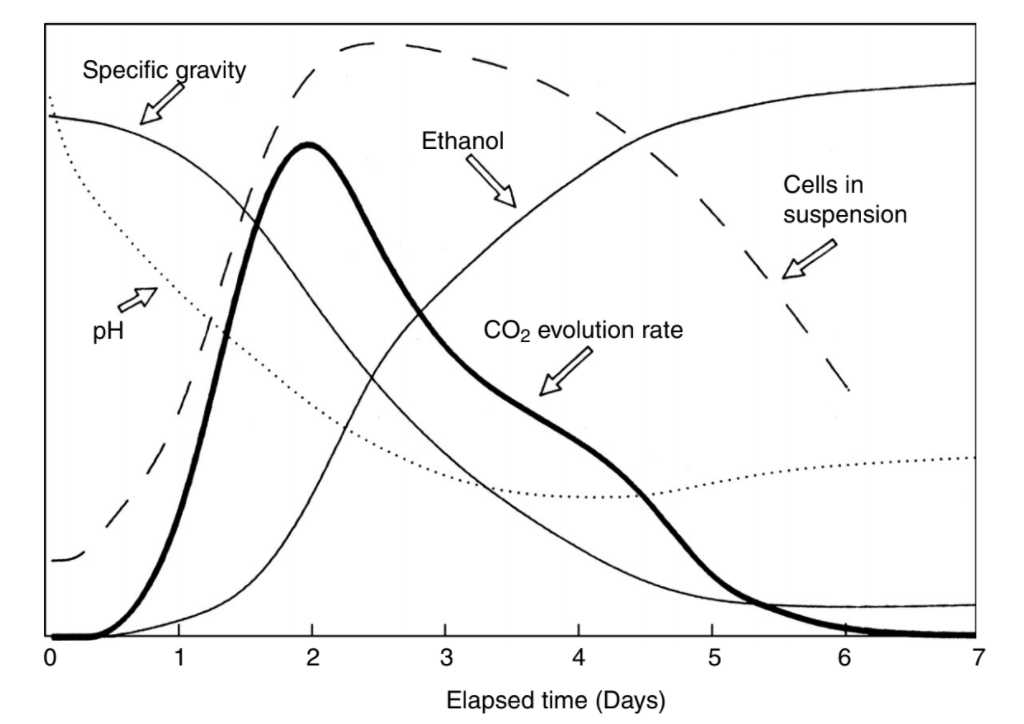
\includegraphics[scale=0.40]{figuras/contexto/variaveis_fermentacao.PNG}
    \captionsource{Gráfico de evolução de variáveis ao longo da fermentação.}{\citeonline{FermentationMunroe}}
    \label{fig:variaveis_fermentacao}
\end{figure}

% \section{Estado da Arte de Sistemas de Produção Artesanal}

% \subsection{Análise de Soluções Existentes}

% % // TODO: Escrever Estado da Arte e Análise de Soluções Existentes



\chapter{Metodologia do Trabalho}


\chapter{Projeto}

\section{Especificação de Requisitos Técnicos}

O protótipo deve ser capaz de monitorar e controlar o processo de fermentação de cervejas, seguindo as configurações de receita definidas pelo usuário. 
Todas as informações coletadas devem ser disponibilizadas ao usuário com a finalidade de possibilitar maior entendimento e reprodutibilidade 
do processo. O projeto foi dividido em dois sistemas: um Hardware, encarregado das medições e controle, e um Software, responsável por exibir informações e estabelecer uma interface com o usuário. A partir dessas premissas, foram determinados os seguintes requisitos para cada um dos sistemas.

\subsection{Sistema Hardware}

\subsubsection{Requisitos funcionais de Hardware}

HW-F-1) O sistema deve monitorar a temperatura (entre 0 e 100 °C), com precisão de 0,5 °C e intervalo de 1 minuto.

HW-F-2) O sistema deve monitorar o pH em intervalo de 1 minuto.

HW-F-3) O sistema deve monitorar a densidade relativa (entre 1,000 e 1,150), com precisão de 0,001 em relação à água a 20°C e intervalo de 1 minuto.

HW-F-4) O sistema deve controlar a temperatura de até 20 Litros de mosto em fermentação, com desvio máximo de 0,5°C em relação ao valor definido pelo usuário e diferença máxima de 10°C em relação ao ambiente.

HW-F-5) O sistema deve seguir o perfil de controle (temperatura x tempo) definido pelo usuário no Software.

HW-F-6) Os dados monitorados devem ser enviados para o Software a cada 5 minutos por meio de rede sem fio.

\subsubsection{Requisitos não funcionais de Hardware}

HW-NF-1) O sistema deve ser acoplável a fermentadores de até 20 Litros disponíveis no mercado.

HW-NF-2) Em caso de perda de conexão com o Software, o sistema deve tentar enviar os dados ainda não enviados a cada ciclo de envio.

HW-NF-3) Caso o sistema tenha uma oscilação no fornecimento de energia, ele deve ser capaz de voltar ao funcionamento normal.

HW-NF-4) Os dados monitorados devem ser armazenados temporariamente, por no mínimo 15 dias, no Hardware.

\subsection{Sistema Software}

\subsubsection{Requisitos funcionais de Software}

SW-F-1) O sistema deve fornecer acesso ao usuário após identificação com usuário e senha

SW-F-2) O sistema deve fornecer as informações instantâneas das fermentações em progresso.

SW-F-3) O sistema deve permitir acesso às informações históricas de fermentações já realizadas.

SW-F-4) O sistema deve permitir o cadastro de receitas. Uma receita é definida por: identificação, nome, estilo e campo livre para observações. O campo livre pode evoluir para um cadastro padronizado dos ingredientes e processos realizados.

SW-F-5) O sistema deve permitir o cadastro de lotes. Um lote é definido por: identificação, receita utilizada, instante de início da fermentação, instante de fim da fermentação, variáveis personalizadas, perfil de controle e observação.

SW-F-6) O sistema deve permitir o cadastro de perfis de controle. Um perfil de controle é definido por: identificação, nome e temperatura alvo, instante (em relação ao início da fermentação).

SW-F-7) O sistema deve permitir o cadastro de variáveis personalizadas. Uma variável personalizada é definida por: identificador, lote correspondente, chave, valor e instante (em relação ao início da fermentação).

SW-F-8) O sistema deve disponibilizar, para cada lote um gráfico com a evolução de cada variável monitorada ao longo do tempo de fermentação.

SW-F-9) Os dados recebidos pelo Hardware devem ser salvos em banco de dados

SW-F-10) Em caso de perda de conexão com o Hardware, o usuário deve ser notificado por e-mail.

SW-F-11) O sistema deve permitir que o usuário realize o download de seus dados em formato de planilha.

SW-F-12) O sistema deve permitir que o usuário registre seus dispositivos.


\subsubsection{Requisitos não funcionais de Software}

SW-NF-1) As informações de cada usuário são, por padrão, particulares de cada usuário e devem seguir padrões de segurança.

SW-NF-2) As informações instantâneas devem estar disponíveis em até 1 minuto após o recebimento dos dados pelo HW.

SW-NF-3) O sistema deve ser desenvolvido na forma de Web-App, e ser responsivo a dispositivos mobile e computadores.



\section{Projeto de Controle}

\subsection{Modelagem Térmica do Sistema}

O primeiro passo para a implementação do controle de temperatura da fermentação é a modelagem térmica do processo. Nota-se que essa modelagem é bastante complexa pois envolve diversos coeficientes térmicos desconhecidos, devido a composição heterogênea do Mosto com Leveduras. 

O objetivo do sistema é controlar a temperatura do líquido fermentado (solução de mosto e leveduras). O líquido estará dentro de um fermentador, sem entrada de ar dado que a fermentação é anaeróbica e o ar interfere na qualidade do experimento. Para expulsar o $CO_2$ gerado pela fermentação e não permitir a entrada de $O_2$ o fermentador utiliza um Air-Lock, dispositivo que funciona como válvula só permitindo a direção única desse fluxo. O fermentador será embalado em uma manta térmica, com a intenção de evitar a troca térmica com o ambiente.

Na maior parte das receitas, a fermentação ocorre em temperaturas entre 14°C e 20°C, temperaturas muitas vezes inferiores à temperatura do ambiente. Sendo assim, existe a necessidade de criar um sistema que troque calor com o mosto e leveduras mantendo um gradiente de temperatura entre o fermentador e o ambiente constante conforme configuração do usuário. 

Para isso acontecer durante o processo, o calor retirado pela refrigeração deve ser o mesmo que o gerado pela convecção com o ambiente e pelo próprio processo de fermentação, que é exotérmico. 


É importante destacar que o dispositivo irá ter duas funções: a primeira será manter a temperatura do líquido fermentado; a segunda será levar o líquido até determinada temperatura. Ambas as funcionalidades envolvem a capacidade do dispositivo de retirar ou fornecer calor do sistema de forma eficiente e constante. 


\subsection{Transferência de Calor entre Ar e Fermentador}

Nessa modelagem, serão analisados os seguintes elementos: 
\begin{itemize}
    \item Mosto e Leveduras 
    \item Tanque de Fermentação 
    \item Manta Térmica 
\end{itemize}

Nessa dinâmica, considerando que o fermentador vai operar na maior parte do tempo em temperaturas inferiores às do ambiente, o calor vai fazer o seguinte caminho:
\begin{enumerate}
    \item A manta térmica recebe calor do ambiente através da convecção e radiação do ar. 
    \item A manta térmica transfere calor por condução para o fermentador. 
    \item O fermentador transfere calor por condução para o líquido fermentado. 
    \item O líquido fermentado produz calor pelo processo de fermentação (processo exotérmico).
\end{enumerate}

\begin{center}
    \(Ambiente \longrightarrow Manta\;t\acute{e}rmica \longrightarrow Fermentador \longrightarrow Mosto\;e\;leveduras\)
\end{center}



    
Algumas hipóteses foram adotadas visando simplificar o problema: 

\begin{enumerate}
    \item O gradiente de temperatura no interior do Mosto + Leveduras é desprezível; 
    \item O coeficiente de troca de calor por convecção entre o Mosto + leveduras e o tanque é elevados o bastante para que não sejam observadas diferenças de temperatura entre esses elementos; 
    \item O regime é permanente e as propriedades são constantes 
    \item A condução é unidimensional no plano X
    \item A transferência de calor por radiação é desprezível nas superfícies 
    \item Resistências de contato desprezíveis.
\end{enumerate}


As hipóteses 1, 2, 3  podem ser adotadas devido ao horizonte de tempo da fermentação, no qual é necessário manter a mesma temperatura durante dias. As hipóteses 4, 5 e 6 foram adotadas com a intenção de simplificar o problema. A figura \ref{fig:fermentador_controle} exemplifica esse problema.

\begin{figure}[h]
    \centering
    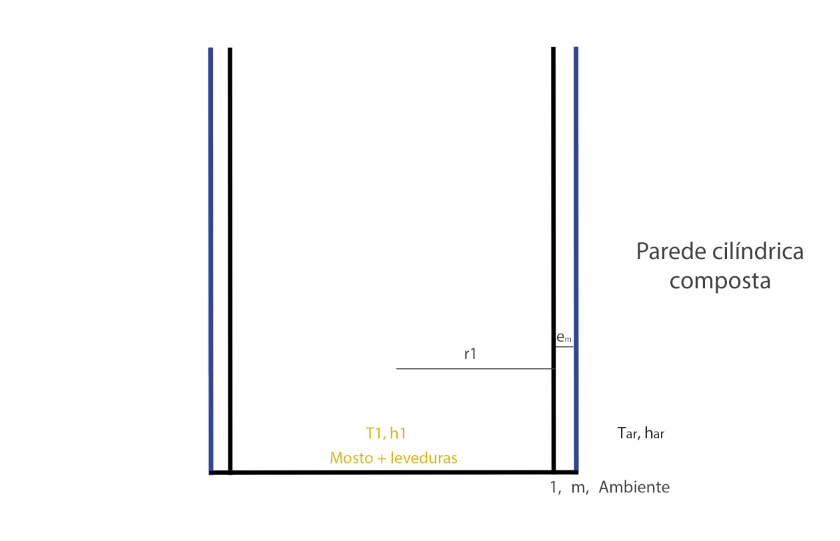
\includegraphics[scale=0.45]{figuras/projeto/controle/fermentador_controle.png}
    \captionsource{Desenho do problema de troca de calor entre o ambiente e fermentador.}{Autores}
    \label{fig:fermentador_controle}
\end{figure}



\subsection{Simulação Térmica}

A Simulação térmica do sistema possui três objetivos:

\begin{enumerate}
    \item Estimar a potência de troca de calor necessária para manter o sistema com 10°C de diferença em relação à temperatura ambiente;
    \item Estimar o tempo morto do sistema para levar o sistema do equilíbrio térmico para uma diferença de 10°C;
    \item Simular um controle PID utilizando uma fonte de calor variável, no caso do sistema real, uma pastilha de Peltier para a sintonização inicial do sistema.
\end{enumerate}

Com esses testes será possível entender se a utilização de pastilhas de Peltier será suficiente para o controle de temperatura.


Foi utilizada a biblioteca Simscape do software Matlab. Essa biblioteca contém blocos que simulam elementos térmicos e funcionam de maneira análoga a um circuito elétrico. No caso, a diferença de temperatura seria equivalente à diferença de potencial elétrico e o calor que circula no sistema seria equivalente a corrente elétrica. As figuras \ref{fig:sim_fonte_calor} a \ref{fig:sim_sensor} representam blocos utilizados.


\begin{figure}[H]
    \centering
    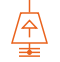
\includegraphics[scale=1.0]{figuras/projeto/controle/fonte_calor.png}
    \caption{Bloco de fonte de calor, que mantém a temperatura em um ponto do circuito constante.}
    \label{fig:sim_fonte_calor}
\end{figure}

\begin{figure}[H]
    \centering
    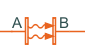
\includegraphics[scale=1.0]{figuras/projeto/controle/conveccao.png}
    \caption{Bloco de transferência de calor por convecção, seguindo a fórmula \(Q = k \cdot A \cdot (T_A - T_B) \)}
    \label{fig:sim_conveccao}
\end{figure}

\begin{figure}[H]
    \centering
    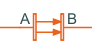
\includegraphics[scale=1.0]{figuras/projeto/controle/radiacao.png}
    \caption{Bloco de transferência de calor por radiação, seguindo a fórmula \(Q = k \cdot A \cdot (T_A^4 - T_B^4) \)}
    \label{fig:sim_radiacao}
\end{figure}

\begin{figure}[H]
    \centering
    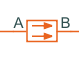
\includegraphics[scale=1.0]{figuras/projeto/controle/conducao.png}
    \caption{Bloco de transferência de calor por condução, seguindo a fórmula \(Q = k \cdot \dfrac{A}{D} (T_A - T_B) \)}
    \label{fig:sim_conducao}
\end{figure}

\begin{figure}[H]
    \centering
    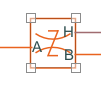
\includegraphics[scale=0.8]{figuras/projeto/controle/sensor_ideal.png}
    \caption{Bloco de sensor de calor ideal}
    \label{fig:sim_sensor}
\end{figure}

\begin{table}[H]
    \begin{center}
        \begin{tabular}{ |c|c| } 
            \hline
            Símbolo & Descrição \\
            \hline
            \(Q\) & Quantidade de Calor \\
            \hline
            \(k\) & Coeficiente de condutividade térmica do material \\
            \hline
            \(A\) & Área normal à transmissão de calor \\
            \hline
            \(D\) & Espessura do material \\
            \hline
            \(T_A, T_B\) & Temperaturas da camada A e B, respectivamente \\
            \hline
        \end{tabular}
        \caption{\label{tab:legenda_blocos} Descrição dos símbolos de trocas de calor referentes às figuras \ref{fig:sim_conveccao} a \ref{fig:sim_conducao}.}
    \end{center}
\end{table}


Com as devidas simplificações justificadas anteriormente, o sistema foi simulado com o circuito da figura \ref{fig:sim_circuito}. A seguir, cada seção de blocos do circuito é descrita em detalhes. A temperatura ambiente adotada na simulação é 25°C e a temperatura do líquido, 15°C.

\begin{figure}[H]
    \centering
    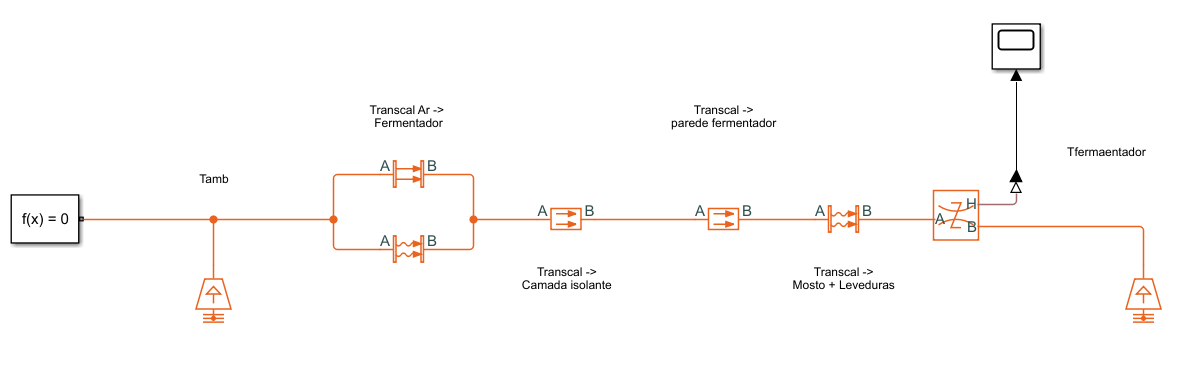
\includegraphics[scale=0.39]{figuras/projeto/controle/sim_circuito.png}
    \captionsource{Circuito de blocos utilizado para a simulação térmica.}{Autores}
    \label{fig:sim_circuito}
\end{figure}


Para a simulação, foi considerado um fermentador cilíndrico com 37 cm de altura e 26 cm de raio. Ele tem paredes de polipropileno com coeficiente térmico de \(0,25 W / m \cdot K\)  e 0,1 cm de espessura. Esse fermentador será encoberto por uma camada de isolante de espuma de poliestireno com coeficiente térmico de  \(0,03 W / m \cdot K\) e 0,2 cm de espessura. O líquido será considerado como água, visando simplificar os cálculos. 


O conjunto de blocos da figura \ref{fig:transcal_amb} representa a transferência de calor entre o ar e a camada isolante que circunda o fermentador. Foram consideradas duas formas de transferência, por convecção e radiação. A área de contato adotada foi \(2 \pi \cdot 0,37 ]cdot 0,263 m^2\), o coeficiente de radiação, \( 5,667 e^{-8} \cdot 0,7 W / m^2 \cdot K^4 \), e o coeficiente de convecção, \(25 W /m^2 \cdot K\) (ar).

\begin{figure}[H]
    \centering
    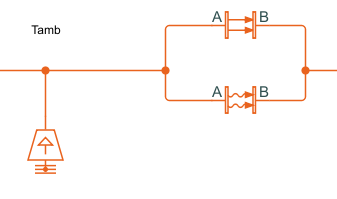
\includegraphics[scale=0.6]{figuras/projeto/controle/transcal_amb.png}
    \caption{Seção do circuito da figura \ref{fig:sim_circuito} referente à transferência de calor entre ambiente e isolamento do fermentador.}
    \label{fig:transcal_amb}
\end{figure}


O bloco da figura \ref{fig:transcal_isolante} representa a transferência de calor por condução entre as paredes do isolante térmico que circunda o fermentador. Foi considerada área de \(2\pi \cdot 0,37 \cdot 0,263 m^2\), espessura de 0,2 cm e coeficiente térmico de condução, \(0.03 W / m \cdot K\).

\begin{figure}[H]
    \centering
    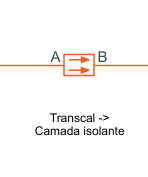
\includegraphics[scale=0.8]{figuras/projeto/controle/transcal_isolante.png}
    \caption{Seção do circuito da figura \ref{fig:sim_circuito} referente à transferência de calor pelo isolamento do fermentador.}
    \label{fig:transcal_isolante}
\end{figure}


A transferência entre extremidades da parede do fermentador é simbolizada pelo bloco da figura \ref{fig:transcal_fermentador}. Para esse bloco, foi adotada área de \(2\pi \cdot 0,37 \cdot 0,261 m^2\), espessura de 0,1 cm e coeficiente térmico de condução, \(0.25 W / m \cdot K\).

\begin{figure}[H]
    \centering
    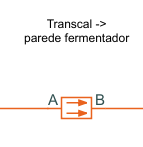
\includegraphics[scale=0.8]{figuras/projeto/controle/transcal_fermentador.png}
    \caption{Seção do circuito da figura \ref{fig:sim_circuito} referente à transferência de calor pelas paredes do fermentador.}
    \label{fig:transcal_fermentador}
\end{figure}


Finalmente, a transferência de calor entre a parede do fermentador e do mosto em fermentação está representado pelo bloco de transferência de calor da figura \ref{fig:transcal_mosto}. Para a simulação foram considerados os valores de área como \(2\pi \cdot 0,37 \cdot 0,261 m^2\) e coeficiente 1000 W / m²·K (considerando a referência da água). 

\begin{figure}[H]
    \centering
    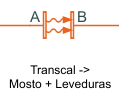
\includegraphics[scale=0.8]{figuras/projeto/controle/transcal_mosto.png}
    \caption{Seção do circuito da figura \ref{fig:sim_circuito} referente à transferência de calor entre paredes do fermentador e mosto em fermentação.}
    \label{fig:transcal_mosto}
\end{figure}


Executando a simulação, a curva de calor resultante (figura \ref{fig:curva_calor}) indica que para manter a temperatura sistema 10°C abaixo do ambiente, é necessário retirar cerca de 57 W de calor do sistema. Esse valor é compatível com a potência máxima das pastilhas de Peltier disponíveis no mercado, que variam entre 90 e 230 W.

\begin{figure}[h]
    \centering
    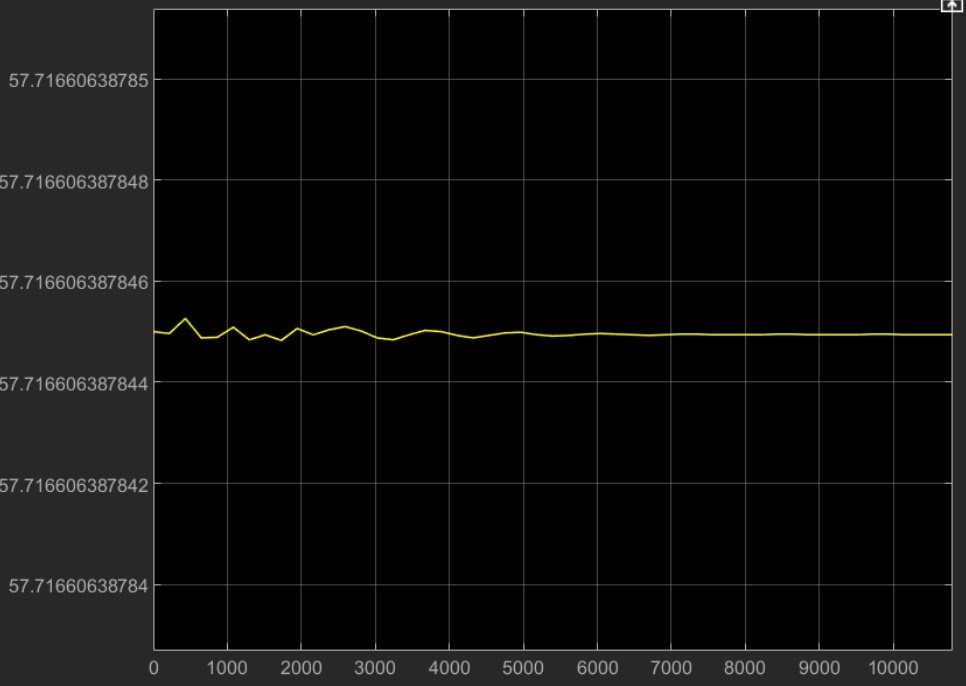
\includegraphics[scale=0.30]{figuras/projeto/controle/curva_calor.jpg}
    \captionsource{Curva de calor obtida a partir da simulação do circuito da figura \ref{fig:sim_circuito}.}{Autores}
    \label{fig:curva_calor}
\end{figure}


Uma segunda simulação foi realizada para determinar o tempo necessário para levar temperatura do sistema do  equilíbrio térmico até uma novo valor. Para isso é ligada uma massa térmica, com o calor específico igual à água de \( 4184 J/K \cdot Kg \), ocupando de 15L do fermentador, e com massa de aproximadamente 15 Kg. O atuador será uma fonte de calor variável, que irá retirar do sistema uma quantidade de calor constante de 57 W. Simulando para intervalo de tempo de 20 horas, foram obtidas as curvas de temperatura (figura \ref{fig:curva_temp}) e quantidade de calor (figura \ref{fig:curva_q}).


\begin{figure}[H]
    \centering
    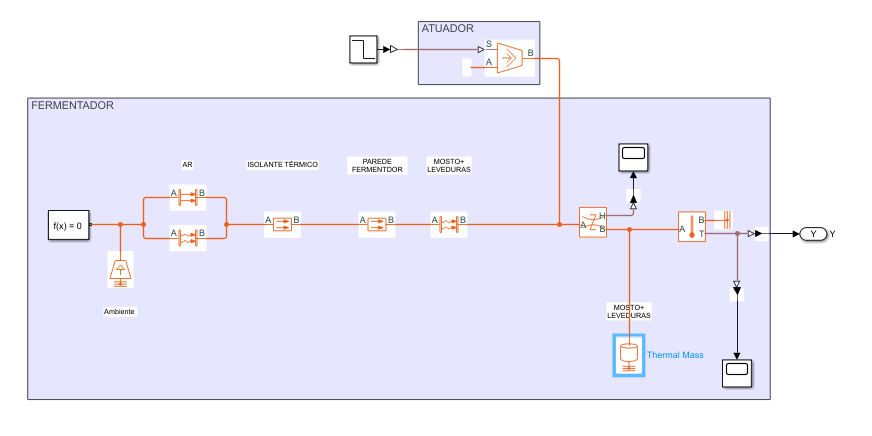
\includegraphics[scale=0.50]{figuras/projeto/controle/circ_atuador.png}
    \captionsource{Circuito térmico completo, com atuador e massa térmica.}{Autores}
    \label{fig:circ_atuador}
\end{figure}


Observando o sistema, conclui-se que o tempo necessário para mover o sistema do equilíbrio térmico para uma temperatura alvo é muito alto e isso pode ser prejudicial nas primeiras horas da fermentação. Dessa forma, é interessante iniciar o processo com a primeira temperatura alvo, o que já é de certa forma realizado na prática, pois a temperatura de início da fermentação deve ser atingida antes do inoculação da levedura e fechamento do fermentador.


\begin{figure}[H]
    \centering
    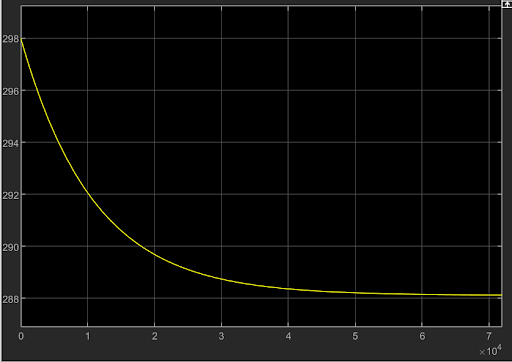
\includegraphics[scale=0.60]{figuras/projeto/controle/curva_temp.png}
    \captionsource{Curva de temperatura em Kelvin por tempo em dezenas de milhares de segundos, obtida da simulação do circuito térmico da figura.}{Autores}
    \label{fig:curva_temp}
\end{figure}

\begin{figure}[H]
    \centering
    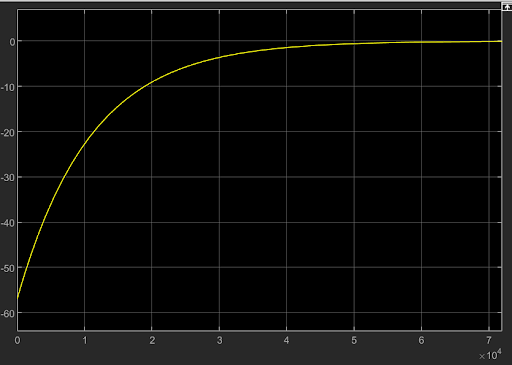
\includegraphics[scale=0.60]{figuras/projeto/controle/curva_q.png}
    \captionsource{Curva de quantidade de calor em Watts por tempo em dezenas de milhares de segundos, obtida da simulação do circuito térmico da figura.}{Autores}
    \label{fig:curva_q}
\end{figure}

\subsection{Dispositivo para Troca de Calor}

Um dos maiores desafios do projeto é criar um sistema que consiga trocar calor de forma eficiente, não seja intrusivo e consiga ser simples o suficiente para ser utilizado por um hobbysta. Conforme anteriormente especificado, a ideia é utilizar placas de peltier para realizar essa troca. A maior vantagem do uso dessas placas é a possibilidade de controlar o calor associado proporcionalmente a quantidade de corrente fornecida ao módulo, através da seguinte equação \ref{eq:qp}. Possibilitando assim o uso de um circuito junto com o microcontrolador para o controle de temperatura.

\begin{equation}
    Q_P = \pi \cdot 1
    \label{eq:qp}
\end{equation}


\subsection{Controle de Temperatura}

Um controlador de malha fechada proporcional interativo derivativo (PID) será utilizado para controlar a temperatura do fermentador. Esse método é amplamente utilizado na indústria, possuindo boa precisão e confiabilidade, além de ser facilmente sintonizado. Inicialmente são definidos parâmetros analógicos e depois é criado o controle digital.

\subsubsection{Controlador PID}

O controlador PID utiliza 3 ações (proporcional, integrativa e derivativa) controlar a planta minimizando o erro. Sua saída pode ser definida pela equação \ref{eq:pid}. A figura \ref{fig:pid} esquematiza a malha de controle.

\begin{equation}
    u(t) = K_pe(t) + K_i  \int_{0}^{t} e(\tau) \, d\tau + K_d\dfrac{de(t)}{\, dt}
    \label{eq:pid}
\end{equation}

Na qual:

\begin{table}[H]
    \begin{center}
        \begin{tabular}{ |c|c| } 
            \hline
            Símbolo   &  Descrição  \\
            \hline
            \(K_p\)   &  ganho proporcional  \\
            \hline
            \(K_i\)   &  ganho integrativo  \\
            \hline
            \(K_d\)   &  ganho derivativo  \\
            \hline
            \(e\)   &  erro  \\
            \hline
            \(t\)   &  tempo  \\
            \hline
            \(\tau\)   &  tempo de integração \\
            \hline
        \end{tabular}
        \caption{\label{tab:variaveis_pid}Descrição das variáveis do controlador PID da Equação \ref{eq:pid}.}
    \end{center}
\end{table}

\begin{figure}[h]
    \centering
    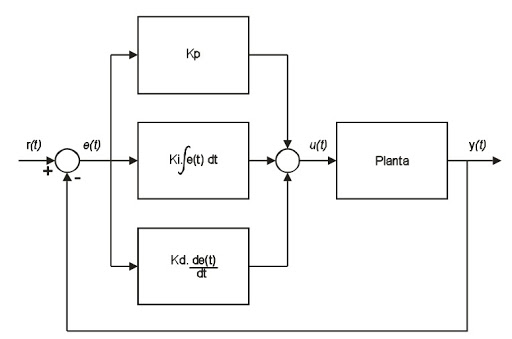
\includegraphics[scale=0.60]{figuras/implementacao/hardware/pid.jpg}
    \caption{Malha de controle PID.}
    \label{fig:pid}
\end{figure}


A ação proporcional do controlador produz um sinal de saída proporcional à amplitude do erro $e(t)$. Essa ação é útil para criar uma resposta equivalente ao tamanho do erro do sistema. A ação integral produz um sinal de saída proporcional à magnitude do erro, dependendo não só do seu valor, mas também da sua duração. Essa ação corrige o erro de off-set gerado pela ação proporcional e acelera a resposta do sistema. Por fim, a ação derivativa produz um sinal de saída proporcional à velocidade de variação do erro. Essa ação melhora a estabilidade e velocidade de resposta do sistema através de uma correção antecipada do erro. 


\subsubsection{Método de Ziegler-Nichols}


Para escolha dos parâmetros de ganho, o método de Ziegler-Nichols foi utilizado. Esse método foi escolhido principalmente pela sua simplicidade e facilidade na sintonização, visto que não é necessário uma modelagem matemática precisa da planta para o seu ajuste. 
A escolha dos parâmetros é feita a partir da observação da resposta do sistema em malha aberta com a aplicação de um degrau. A figura \ref{fig:resposta_sistema} ilustra a curva de resposta do sistema, e a tabela \ref{tab:parametros_ziegler} lista os parâmetros provenientes do método.


\begin{figure}[h]
    \centering
    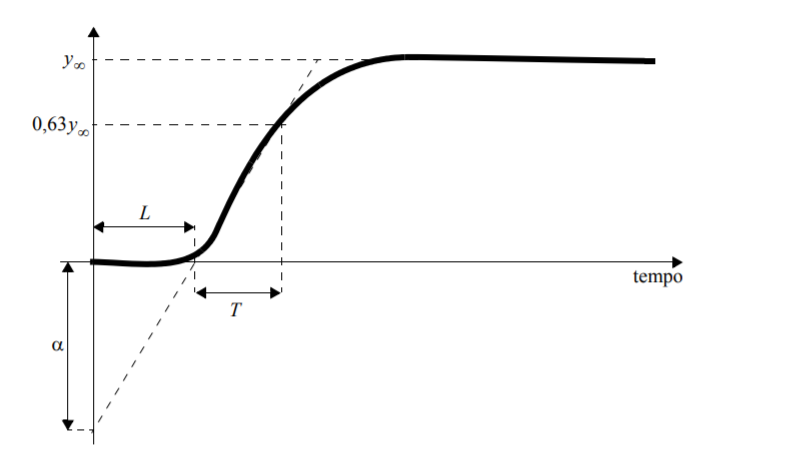
\includegraphics[scale=0.45]{figuras/implementacao/hardware/resposta.png}
    \caption{Responda do Sistema em malha aberta a sinal degrau.}
    \label{fig:resposta_sistema}
\end{figure}

\begin{table}[H]
    \begin{center}
        \begin{tabular}{ |c|c|c|c| } 
            \hline
            Controlador & \(K_p\) & \(T_I\) & \(T_D\) \\
            \hline
            \(P\) & \(1/\alpha\) &  & \\
            \hline
            \(P + I\) & \(0,9/\alpha\) & \(3L\) & \\
            \hline
            \(P + I + D\) & \(1,2/\alpha\) & \(2L\) & \(0,5L\) \\
            \hline
        \end{tabular}
        \caption{\label{tab:parametros_ziegler} Parâmetros do controlador PID seguindo método de Ziegler-Nichols.}
    \end{center}
\end{table}


\subsubsection{Anti Wind-up}

Nesta aplicação, devido a limitações do atuador, é esperado uma saturação na saída. No caso onde o sistema não consegue chegar no setpoint, teremos uma situação chamada de wind-up, na qual, a sua resposta integral irá crescer de forma indefinida. Para evitar problemas no controlador, é necessário a implementação de um sistema anti wind-up, no caso, a ação escolhida será congelar a ação do controlador em caso de saturação.  



\section{Projeto de Hardware}

% // TODO: Especificações técnicas em tabelas

Com base nos requisito, foram determinados os principais componentes do projeto
para o controle e monitoramento do sistema

\subsection{Microcontrolador}

% // TODO: Atualizar para Wemos D1
O microcontrolador Arduino Uno R3 é versátil e ideal para a prototipagem e será
utilizado como microcontrolador do projeto. O mesmo possui portas i/o analógicas e
digitais, fontes de alimentação de 3,3V/5V e é programado na linguagem C.

% \ref{fig:wemos}
\begin{figure}[h]
    \centering
    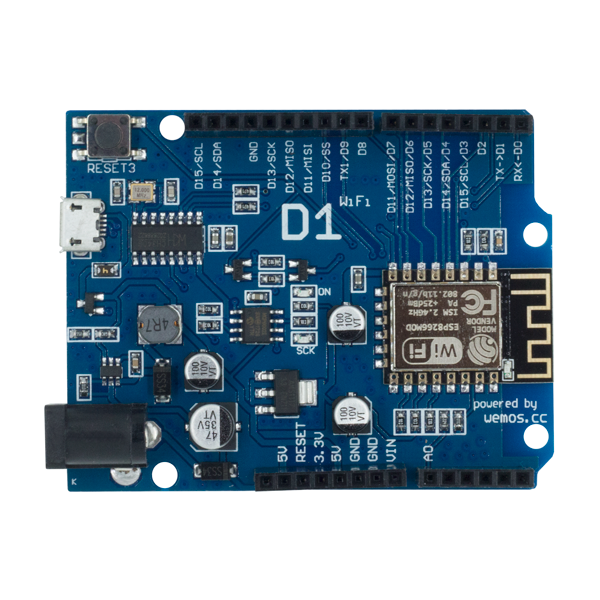
\includegraphics[scale=0.45]{figuras/projeto/hardware/wemos_d1.png}
    \caption{Wemos D1}
    \label{fig:wemos}
\end{figure}

\subsection{Critérios de Escolha dos Sensores}

A definição dos sensores a serem utilizados se baseou nos seguintes critérios, em ordem de importância:

\begin{itemize}
    \item Faixa de operação compatível com os requisitos e especificidades do sistema
    \item Disponibilidade no mercado brasileiro
    \item Compatibilidade com o Arduino
    \item Custo de aquisição
\end{itemize}

O primeiro critério é trivial, e deve ser eliminatório em qualquer avaliação. O critério de disponibilidade no mercado brasileiro teve essa classificação pelo desejo de se adquirir e trabalhar com os sensores o mais rápido possível e mitigar o risco com atrasos devido a importações e falta de estoque. A compatibilidade com o Arduino exprime quão diretamente um sensor pode ser utilizado, principalmente em relação a alimentação, sendo preferíveis sensores que tenham tensões de entrada em comum com o microcontrolador, i.e., 3,3 ou 5V. Finalmente, custos de aquisição menores são preferíveis.

\subsection{Sensor de Temperatura}

Para a medição de temperatura o sensor escolhido foi o circuito integrado DS18B20 (Figura \ref{fig:ds18b20}) com uma vedação impermeável. É um sensor que atende as especificações e é amplamente utilizado em conjunto com o Arduino e microcontroladores semelhantes, e possui alta disponibilidade no mercado a um baixo custo, sendo comercializado em uma versão impermeável, muita prática para esse projeto. A leitura da temperatura pelo microcontrolador é realizada por apenas um fio de dados, utilizando a interface One-Wire. 

Ficha técnica:
\begin{itemize}
    \item Tensão de operação: 3-5,5V
    \item Faixa de medição: -55°C a +125°C
    \item Precisão: ±0.5°C entre -10°C e +85°C
    \item Ponta de aço inoxidável
\end{itemize}

\begin{figure}[h]
    \centering
    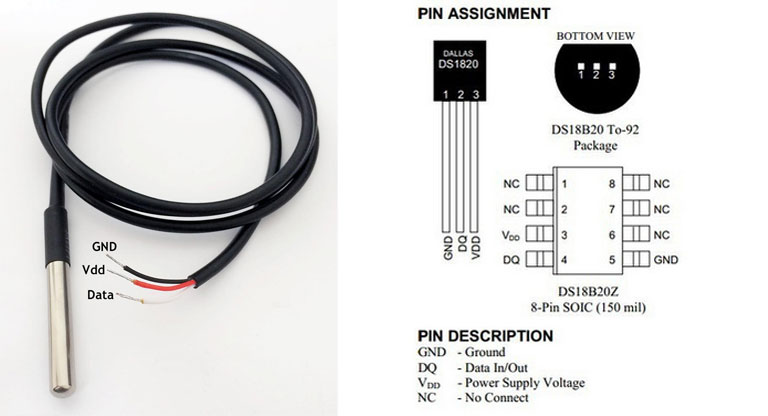
\includegraphics[scale=0.50]{figuras/projeto/hardware/ds18b20.jpg}
    \caption{Sensor DS18B20}
    \label{fig:ds18b20}
\end{figure}

\subsection{Sensor de Densidade Relativa}

A medição da densidade relativa é menos trivial pela ausência de sensores completos comercializados a baixo custo. Quando não é automatizada, a medição é comumente  realizada com auxílio de um densímetro ou um refratômetro, que medem a densidade relativa e a concentração de açúcar dissolvido em graus Brix, respectivamente. Ambas as ferramentas requerem interação humana e a extração de uma pequena amostra da solução, aproximadamente 100 a 250ml e algumas gotas, respectivamente.


Quanto a medição automática e contínua da densidade relativa, Boulton e Quain \cite{BoultonQuain} apresentam algumas formas de medir a grandeza, destacam-se: a utilização de sensores de pressão posicionados em diferentes alturas do fermentador, e computando a diferença de pressões medidas; e utilizando um sensor ultrassônico,  medindo o tempo que um pulso leva para ser transmitido entre dois pontos fixos, entremeado pela solução. 


Em pesquisa por soluções existentes no mercado, a abordagem de dois produtos são dignas de consideração: o Beer Bug utiliza uma célula de carga para medir o empuxo sofrido por um peso submerso na solução, e o Plaato, que utiliza a medição do gás carbônico expelido durante a fermentação para calcular indiretamente a densidade relativa.


Dentre as opções listadas, a medição por diferença de pressões e empuxo foram selecionadas para serem adotadas em primeiro momento no projeto, com prioridade da primeira. Essas são as soluções que aparentam apresentar menor complexidade na medição e maior facilidade na calibração para obtenção de resultados consistentes.


As opções listadas são discutidas a seguir, contemplando as especificações necessárias para cada sensor, e os modelos escolhidos para utilização no projeto.

\subsubsection{Medição por diferença de pressão} 

Esse método se baseia no conceito de pressão estática \(P_{estatica}\), que é pode ser calculda para um determinado ponto em um fluido como o produto da densidade \(\rho\) desse fluido, da aceleração gravitacional \(g\), e da altura \(h\) da coluna de líquido sobre o ponto escolhido.

\begin{equation}
P_{estatica} = \rho \cdot g \cdot h
\end{equation}

Consequentemente, considerando a densidade homogênea e a variação da aceleração gravitacional desprezível, a diferença de pressão entre dois pontos em diferentes alturas desse fluido, é:

\begin{equation}
\Delta P = \rho \cdot g \cdot \Delta h
\end{equation}

Dessa forma, mantendo a diferença de alturas \(\Delta h\) fixa e conhecida, é simples inferir o valor da densidade a partir da medida da diferença de pressão medida pelo sensor.


Seguindo a especificação do requisito HW-F-3, o sistema deve ser capaz de medir densidades relativas de 1,000 e 1,150, em relação à água a 20 °C, o que corresponde a uma faixa entre 998,203 e 1147,933 kg/m³. Considerando a aceleração gravitacional 9.807 m/s² e uma distância de 20 cm entre os dois pontos medidos (o que é razoável para fermentadores pequenos, até 50L), a faixa de operação do sensor de diferencial de pressão deve ser, em diferentes unidades comerciais:

\begin{table}[H]
    \begin{center}
        \begin{tabular}{ |c|c|c|c| } 
            \hline
            & N/m² ou Pa & bar & psi \\
            \hline
            Valor Mínimo & 1957,805 & 0,019578 & 0,284 \\ 
            \hline
            Valor Máximo & 2251,476 & 0,022515 & 0,327 \\ 
            \hline
        \end{tabular}
        \caption{\label{tab:densidades}Diferenças de pressão esperadas para cálculo da densidade relativa durante a fermentação.}
    \end{center}
\end{table}

Para obter a precisão de 1 milésimo de densidade relativa, o sensor necessita de uma precisão de aproximadamente 0,1\%.


A partir das especificações, foram buscados os sensores disponíveis no mercado, principalmente os produzidos pela Mouser Electronics (https://br.mouser.com/). Seguindo os critérios definidos, o modelo escolhido foi o MPXV7002DP (Figura \ref{fig:MPXV7002DP}), que possui as seguintes especificações:

\begin{itemize}
\item Faixa de medição: -0.3 a +0.3 psi
\item Precisão: 2,5\%
\item Tensão de alimentação: 5V
\end{itemize}

Apesar do sensor não apresentar uma precisão adequada, acreditamos que o uso da média de diversas medidas e calibração com algumas medidas feitas pelo usuário podem propiciar resultados satisfatórios.

\begin{figure}[h]
    \centering
    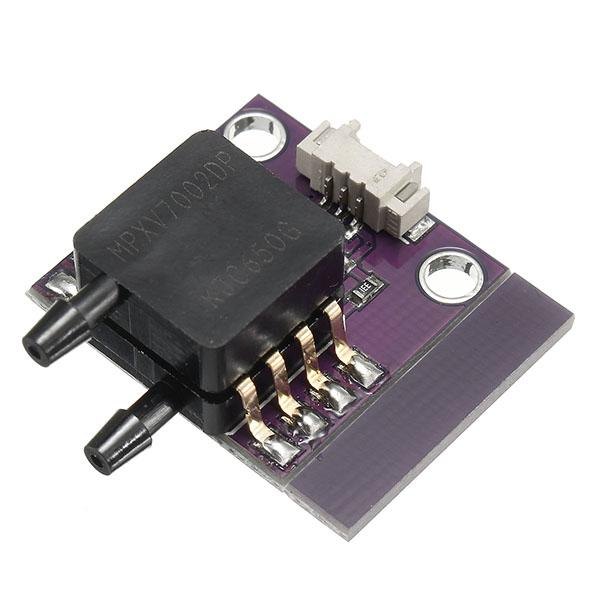
\includegraphics[scale=0.35]{figuras/projeto/hardware/MPXV7002DP.jpg}
    \caption{Sensor de diferença de pressão MPXV7002DP}
    \label{fig:MPXV7002DP}
\end{figure}


\subsubsection{Medição por Empuxo}

O empuxo hidrostático \(E\) sofrido por um corpo submerso em um fluido é expresso pelo produto entre da densidade \(\rho_f\) do fluido, o volume submerso \(V_f\) do corpo, e da aceleração da gravidade \(g\): 

\begin{equation}
    E = \rho_f \cdot V_f \cdot g
\end{equation}

Naturalmente, o corpo também sofre ação da força gravitacional \(P\), que é definida pelo produto da massa \(m\) do corpo pela aceleração gravitacional \(g\):

\begin{equation}
    P = mg
\end{equation}

As duas forças atuam em sentidos opostos (como ilustrado na figura a seguir), de forma que, utilizando uma célula de carga conectada por meio de um fio a um corpo, é possível notar uma diferença no “peso natural” do objeto submerso, que é igual a força resultante entre a força gravitacional e o empuxo. Esse é o conceito de uma balança hidrostática.

\begin{figure}[h]
    \centering
    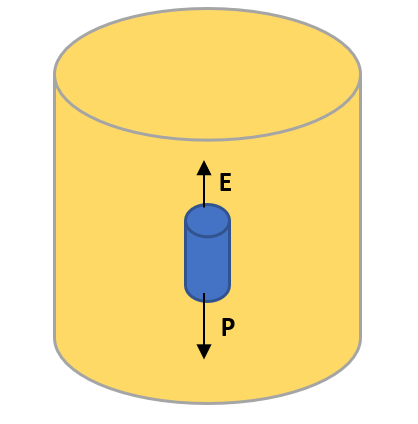
\includegraphics[scale=0.35]{figuras/projeto/hardware/empuxo.PNG}
    \caption{Representação de um corpo (azul) submerso em um fluido (amarelo) e das forças gravitacional e de empuxo}
    \label{fig:empuxo}
\end{figure}

Considerando um corpo de massa 250g e volume de 125cm³ arbitrários, e a variação de densidade especificada, uma célula de carga adequada para o projeto deve ser capaz de medir massas entre 112,75 e 125,22g, com precisão mínima de aproximadamente 0,125g. Nota-se que é desejável um corpo mais denso que o fluido para que ele fique completamente submerso, facilitando aplicação da relação do empuxo. O sensor ZHIPU-200g (Figura \ref{fig:ZHIPU-200g}) foi escolhido, medindo entre 0 a 200g, com precisão de 0,1g.


\begin{figure}[h]
    \centering
    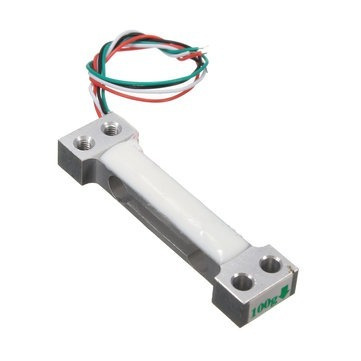
\includegraphics[scale=0.40]{figuras/projeto/hardware/ZHIPU-200g.jpg}
    \caption{Sensor de carga ZHIPU-200g}
    \label{fig:ZHIPU-200g}
\end{figure}


\subsection{Sensor de pH}

Para a medição de pH o sensor escolhido foi o E-201-C (Figura \ref{fig:E-201-C}) com uma placa condicionadora que permite interface direta com o microcontrolador. Assim como o DS18B20, é um sensor amplamente utilizado em conjunto com o Arduino e facilmente encontrado no mercado nacional. A comunicação com o microcontrolador é realizada por comunicação serial, utilizando os protocolos UART ou I2C.


Ficha técnica:
\begin{itemize}
    \item Tensão de operação: 5V;
    \item Temperatura de operação: 0°C a 60°C;
    \item Tempo de resposta: 5s;
    \item Tempo de sedimentação: 60s;
    \item Faixa de medição: pH de 0 a 14
\end{itemize}

\begin{figure}[h]
    \centering
    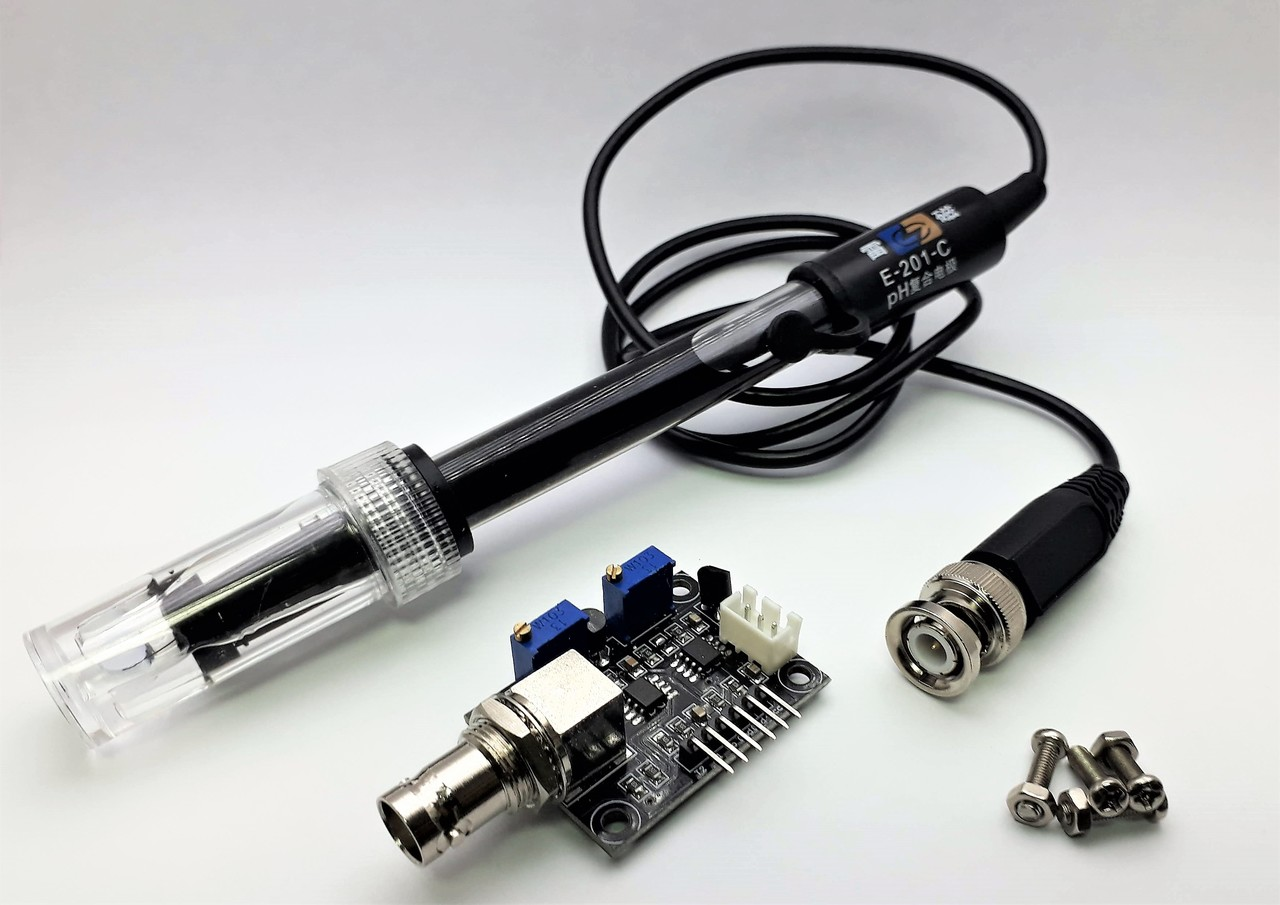
\includegraphics[scale=0.15]{figuras/projeto/hardware/E-201-C.jpg}
    \caption{Sensor de pH E-201-C}
    \label{fig:E-201-C}
\end{figure}


\subsection{Atuador de Temperatura}

Para a montagem do nosso dispositivo que realiza trocas de calor com o fermentador, as células termoelétricas de Peltier se mostraram uma boa opção. Elas são versáteis, possuem a capacidade de esfriar ou aquecer o fermentador dependendo do sentido da corrente aplicada em seus terminais e fornecem calor proporcionalmente a corrente fornecida ao sistema.


A célula é constituída por duas chapas de material isolante com um material condutor entre elas, como é esquematizado na Figura \ref{fig:esquema_peltier}. Quando uma diferença de tensão é aplicada entre os terminais da célula, o movimento dos semicondutores de tipo “n” e “p” transforma a energia elétrica em energia térmica, criando um fluxo de calor que aquece uma célula e esfria outra. Em um semicondutor do tipo-n, o calor é absorvido próximo ao terminal negativo e rejeitado próximo ao terminal positivo, já em um semicondutor do tipo-p o processo se dá de maneira inversa. Como os pares tipo “n” e “p” tem características diferentes, é possível alterar o fluxo de calor dependendo do sentido da corrente.


\begin{figure}[h]
    \centering
    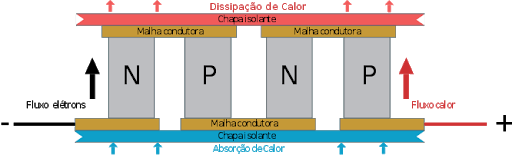
\includegraphics[scale=0.60]{figuras/projeto/hardware/peltier.png}
    \caption{Esquema de uma célula de Peltier}
    \label{fig:esquema_peltier}
\end{figure}


Um exemplo de aplicação comercial das células de Peltier para controle da temperatura de fermentação, pode ser observada no produto desenvolvido pela Brew Jacket, que consiste em uma célula de Peltier conectada em lado a uma haste de transferência de calor, que fica em contato com a solução, e ao outro lado, a um dissipador de calor e ventoinha, que ficam externos ao fermentador. O produto recomenda a utilização de uma capa térmica sobre o fermentador para aumentar a eficiência do controle de temperatura.


Uma alternativa, ainda se utilizando a célula de peltier, é realizar a troca de calor com a solução pela parede do fermentador, de forma menos invasiva e com menores riscos de contaminação, mas gerando uma dependência maior à geometria e material do fermentador. Opções a serem estudadas nesta alternativa são a utilização das células em contato próximo à parede do fermentador; e a construção de um pequeno sistema que utilize um líquido circulando por serpentinas em torno ao fermentador, com as células  controlando a temperatura do líquido.

% // TODO: Projeto de Montagem
% // TODO: Diagrama do Circuito


\section{Projeto de Software}

A partir dos Requisitos Técnicos levantados, foi realizado o projeto de software. O projeto se iniciou com a definição de casos de uso a serem implementados, de forma a satisfazer os requisitos técnicos, em conjunto o diagrama de casos de uso definido pela UML foi elaborado para prover apresentação visual. Em seguida, as informações que devem ser armazenadas pelo sistema foram levantadas e a relação entre elas foi estabelecida, sendo representada no diagrama de entidade-relacionamento. O passo seguinte foi a definição da arquitetura de software do sistema.

No projeto a arquitetura de microsserviços foi escolhida como padrão para o sistema. Essa arquitetura define padrões de modularização do sistema em componentes pequenos e altamente especializados, conferindo facilidades de manutenção e escalabilidade em contraste com a arquitetura de monólito. Em contrapartida, o sistema é mais complexo de se implementar e implantar, devido a separação dos módulos, contudo, considerando o desejo de continuar este projeto após a entrega e os padrões de mercado atuais a abordagem de microsserviços é considerada a mais adequada. 

Definida a arquitetura, cada módulo do sistema foi especificado e foi elaborado o diagrama de componentes, definido pela UML, para ilustrar os pontos de comunicação e componentização da solução completa. Nessa etapa foram definidas as tecnologias a serem empregadas em cada módulo, a justificativa das escolhas é apresentada após o detalhamento dos componentes da arquitetura de software. O projeto de implantação foi então realizado, com planejamento da disponibilização do sistema de software com ferramentas de computação de nuvem disponíveis no mercado.

\subsection{Especificação dos Casos de Uso}

Na definição dos casos de uso do projeto foram definidos dois atores que interagem com o sistema de software a ser desenvolvido, identificados como 
usuário e dispositivo. O usuário representa o utilizador humano do sistema a ser desenvolvido, responsável por todas as interações humanas necessárias. 
O usuário se comunica com o sistema por duas interfaces, uma aplicação web, que se comunica diretamente com o sistema, e um aplicativo para smartphone, necessário para configurações iniciais do dispositivo. O dispositivo representa o sistema hardware de controle e monitoramento, também desenvolvido neste projeto. Em relação ao sistema de software, ele é tratado como um ator com suas devidas interações; seu projeto e especificações são discutidos na seção destinado ao projeto de hardware.

Segue a especificação dos casos de uso em si, contendo a identificação de cada caso de uso, sua breve descrição, enumeração dos passos que o definem e 
listagem dos requisitos técnicos relacionados ao caso de uso. Com caráter ilustrativo, o Diagrama de Casos de Uso da UML é apresentado na figura \ref{fig:diagrama_caso_de_usos}.

\subsubsection*{UC - 1: Registro de Dispositivo} 

Descrição: ao obter um novo dispositivo, o usuário deve configurar seu acesso à rede Wi-Fi e registrá-lo, de modo que o sistema reconheça que aquele 
dispositivo pertence ao usuário.
\begin{enumerate}
    \item Usuário acessa aplicativo em seu smartphone
    \item Sistema autentica acesso do usuário
    \item Aplicativo se conecta ao dispositivo
    \item Usuário informa configurações da rede Wi-Fi
    \item Aplicativo envia informações da rede para dispositivo
    \item Dispositivo se conecta na rede e se prepara para receber mensagens do sistema
    \item Aplicativo envia informações do dispositivo para o sistema
    \item Sistema cadastra informações do dispositivo e usuário
\end{enumerate}
Requisito relacionado: SW-F-12

\subsubsection*{UC - 2: Cadastro de Receitas}
Descrição: fluxo de cadastro de receitas.
\begin{enumerate}
    \item Usuário acessa tela de listagem de receitas
    \item Sistema exibe todas as receitas referentes ao usuário
    \item Usuário seleciona opção “Criar Receita” e acessa tela de cadastro de receita
    \item Usuário informa nome, estilo e observações da receita e clica em “Salvar”
    \item Sistema cadastra a receita no banco de dados
\end{enumerate}
Requisito relacionado: SW-F-4

\subsubsection*{UC - 3: Cadastro de Lotes}
Descrição: fluxo de cadastro de lotes, perfis de controle e associação de lote a um dispositivo.
\begin{enumerate}
    \item Usuário acessa tela de listagens de receitas
    \item Sistema exibe todas as receitas referentes ao usuário
    \item Usuário escolhe uma receita e seleciona a opção “Criar Lote”, e acessa a tela de cadastro de lote
    \item Sistema carrega listagem de perfis de controle já cadastrados e dispositivos do usuário
    \item Usuário informa identificação e observações do lote
    \item Usuário escolhe um perfil de controle já existente ou cria um novo perfil, informando uma identificação e cada um dos passos de controle (instante e valor alvo de temperatura)
    \item Usuário seleciona qual dispositivo irá controlar a produção do lote
    \item Usuário clica em “Salvar”
    \item Sistema cadastra lote, perfil de controle (caso novo), associação de lote e perfil de controle, e associação de lote e dispositivo
    \item Sistema envia informações do lote para dispositivo selecionado
\end{enumerate}
Requisitos relacionados: SW-F-5 e SW-F-6.

\subsubsection*{UC - 4: Envio das informações do Lote para Dispositivo}
Descrição: fluxo de envio das informações do lote para o dispositivo associado ao controle daquele lote.
\begin{enumerate}
    \item Dispositivo recebe informações do lote que foi associado por tópico de mensagens
    \item Dispositivo salva informações localmente
    \item Quando pronto, dispositivo inicia rotina de monitoramento e controle
\end{enumerate}    
Requisito relacionado: HW-F-5

\subsubsection*{UC - 5: Envio das informações do Dispositivo para o Sistema}
Descrição: fluxo de envio das informações obtidas pelo monitoramento do processo pelo dispositivo para o sistema.
\begin{enumerate}
    \item Dispositivo envia dados coletados para o sistema
    \item Sistema processa dados e salva informações no banco de dados
\end{enumerate}    
Requisitos relacionados: HW-F-6, SW-F-9

\subsubsection*{UC - 6: Visualização das Informações dos Lotes}
Descrição: fluxo para visualização das informações gerais e de evolução dos lotes correntes e passados
\begin{enumerate}
    \item Usuário acessa tela de listagem dos lotes
    \item Sistema exibe todas os lotes referentes ao usuário
    \item Usuário escolhe um lote e seleciona a opção “Ver Informações”, acessando a tela de informações do lote
    \item Sistema exibe informações gerais sobre o lote, como identificação, receita, observações, status, data de início, data de término, densidades relativas inicial e final/atual, estimativa de teor alcoólico, pH final/atual, temperatura final/atual.
    \item Sistema exibe um gráfico com as variáveis monitoradas em relação ao tempo
    \item Caso usuário clique em “Baixar Dados”, sistema efetua o download dos dados do gráfico em arquivo de texto
\end{enumerate}    
Requisitos relacionados: SW-F-2, SW-F-3, SW-F-8, SW-F-11

\begin{figure}[ht]
    \centering
    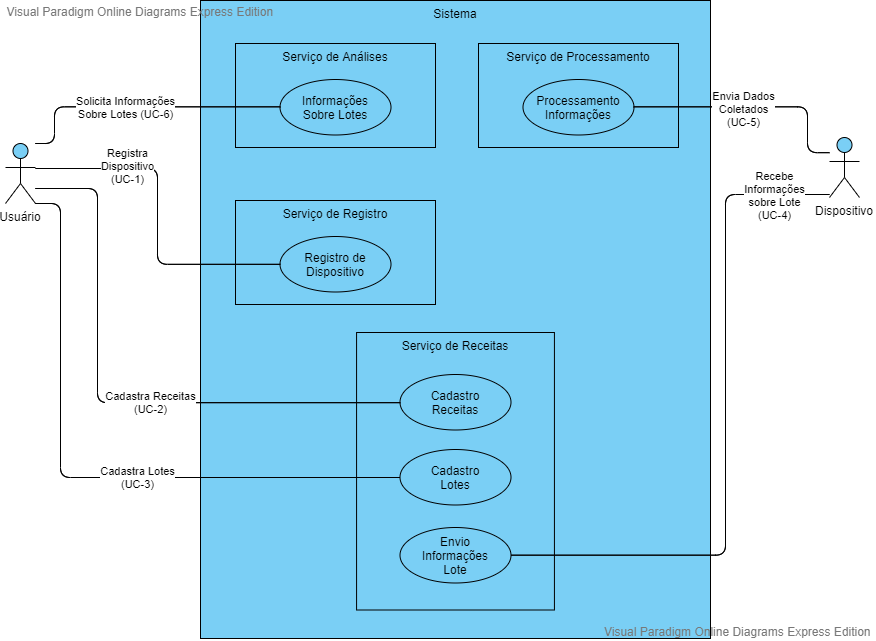
\includegraphics[scale=0.45]{figuras/projeto/software/diagrama_casos_de_uso.png}
    \caption{Diagrama de Casos de Uso.}
    \label{fig:diagrama_caso_de_usos}
\end{figure}

\subsection{Modelo de Entidade-Relacionamento}

O Modelo Entidade Relacionamento descreve como as informações são organizada no sistema e como o banco de dados do sistema é estruturado. 
Cada entidade no modelo representa um tipo de informação que é produzida e consumida pelo sistema, na execução dos casos de uso. 

Todas as informações são armazenadas em um banco de dados relacional, dividido em schemas que atuam como partições de dados em diferentes domínios. 
Foram definidos três domínios, traduzidos em schemas no banco de dados, para os dados: user, recipe e control. O schema user contém as informações 
referentes aos usuários e dispositivos do sistema; o domínio recipe contempla as entidades relacionadas às receitas e lotes de produção, assim como 
os dados coletados em cada execução de uma receita; e o schema control, por fim, os perfis de controle que são seguidos pelo dispositivo durante 
seu funcionamento. A separação das entidades em domínios é importante na arquitetura de microsserviços para assegurar que cada serviço tenha 
controle apenas às informações de sua competência. 

A definição das entidades e seus relacionamentos é ilustrada pelo Diagrama Entidade Relacionamento da figura \ref{fig:diagrama_entidade_relacionamento}, com destaque em cor para cada um 
dos schemas determinados.

\begin{figure}[ht]
    \centering
    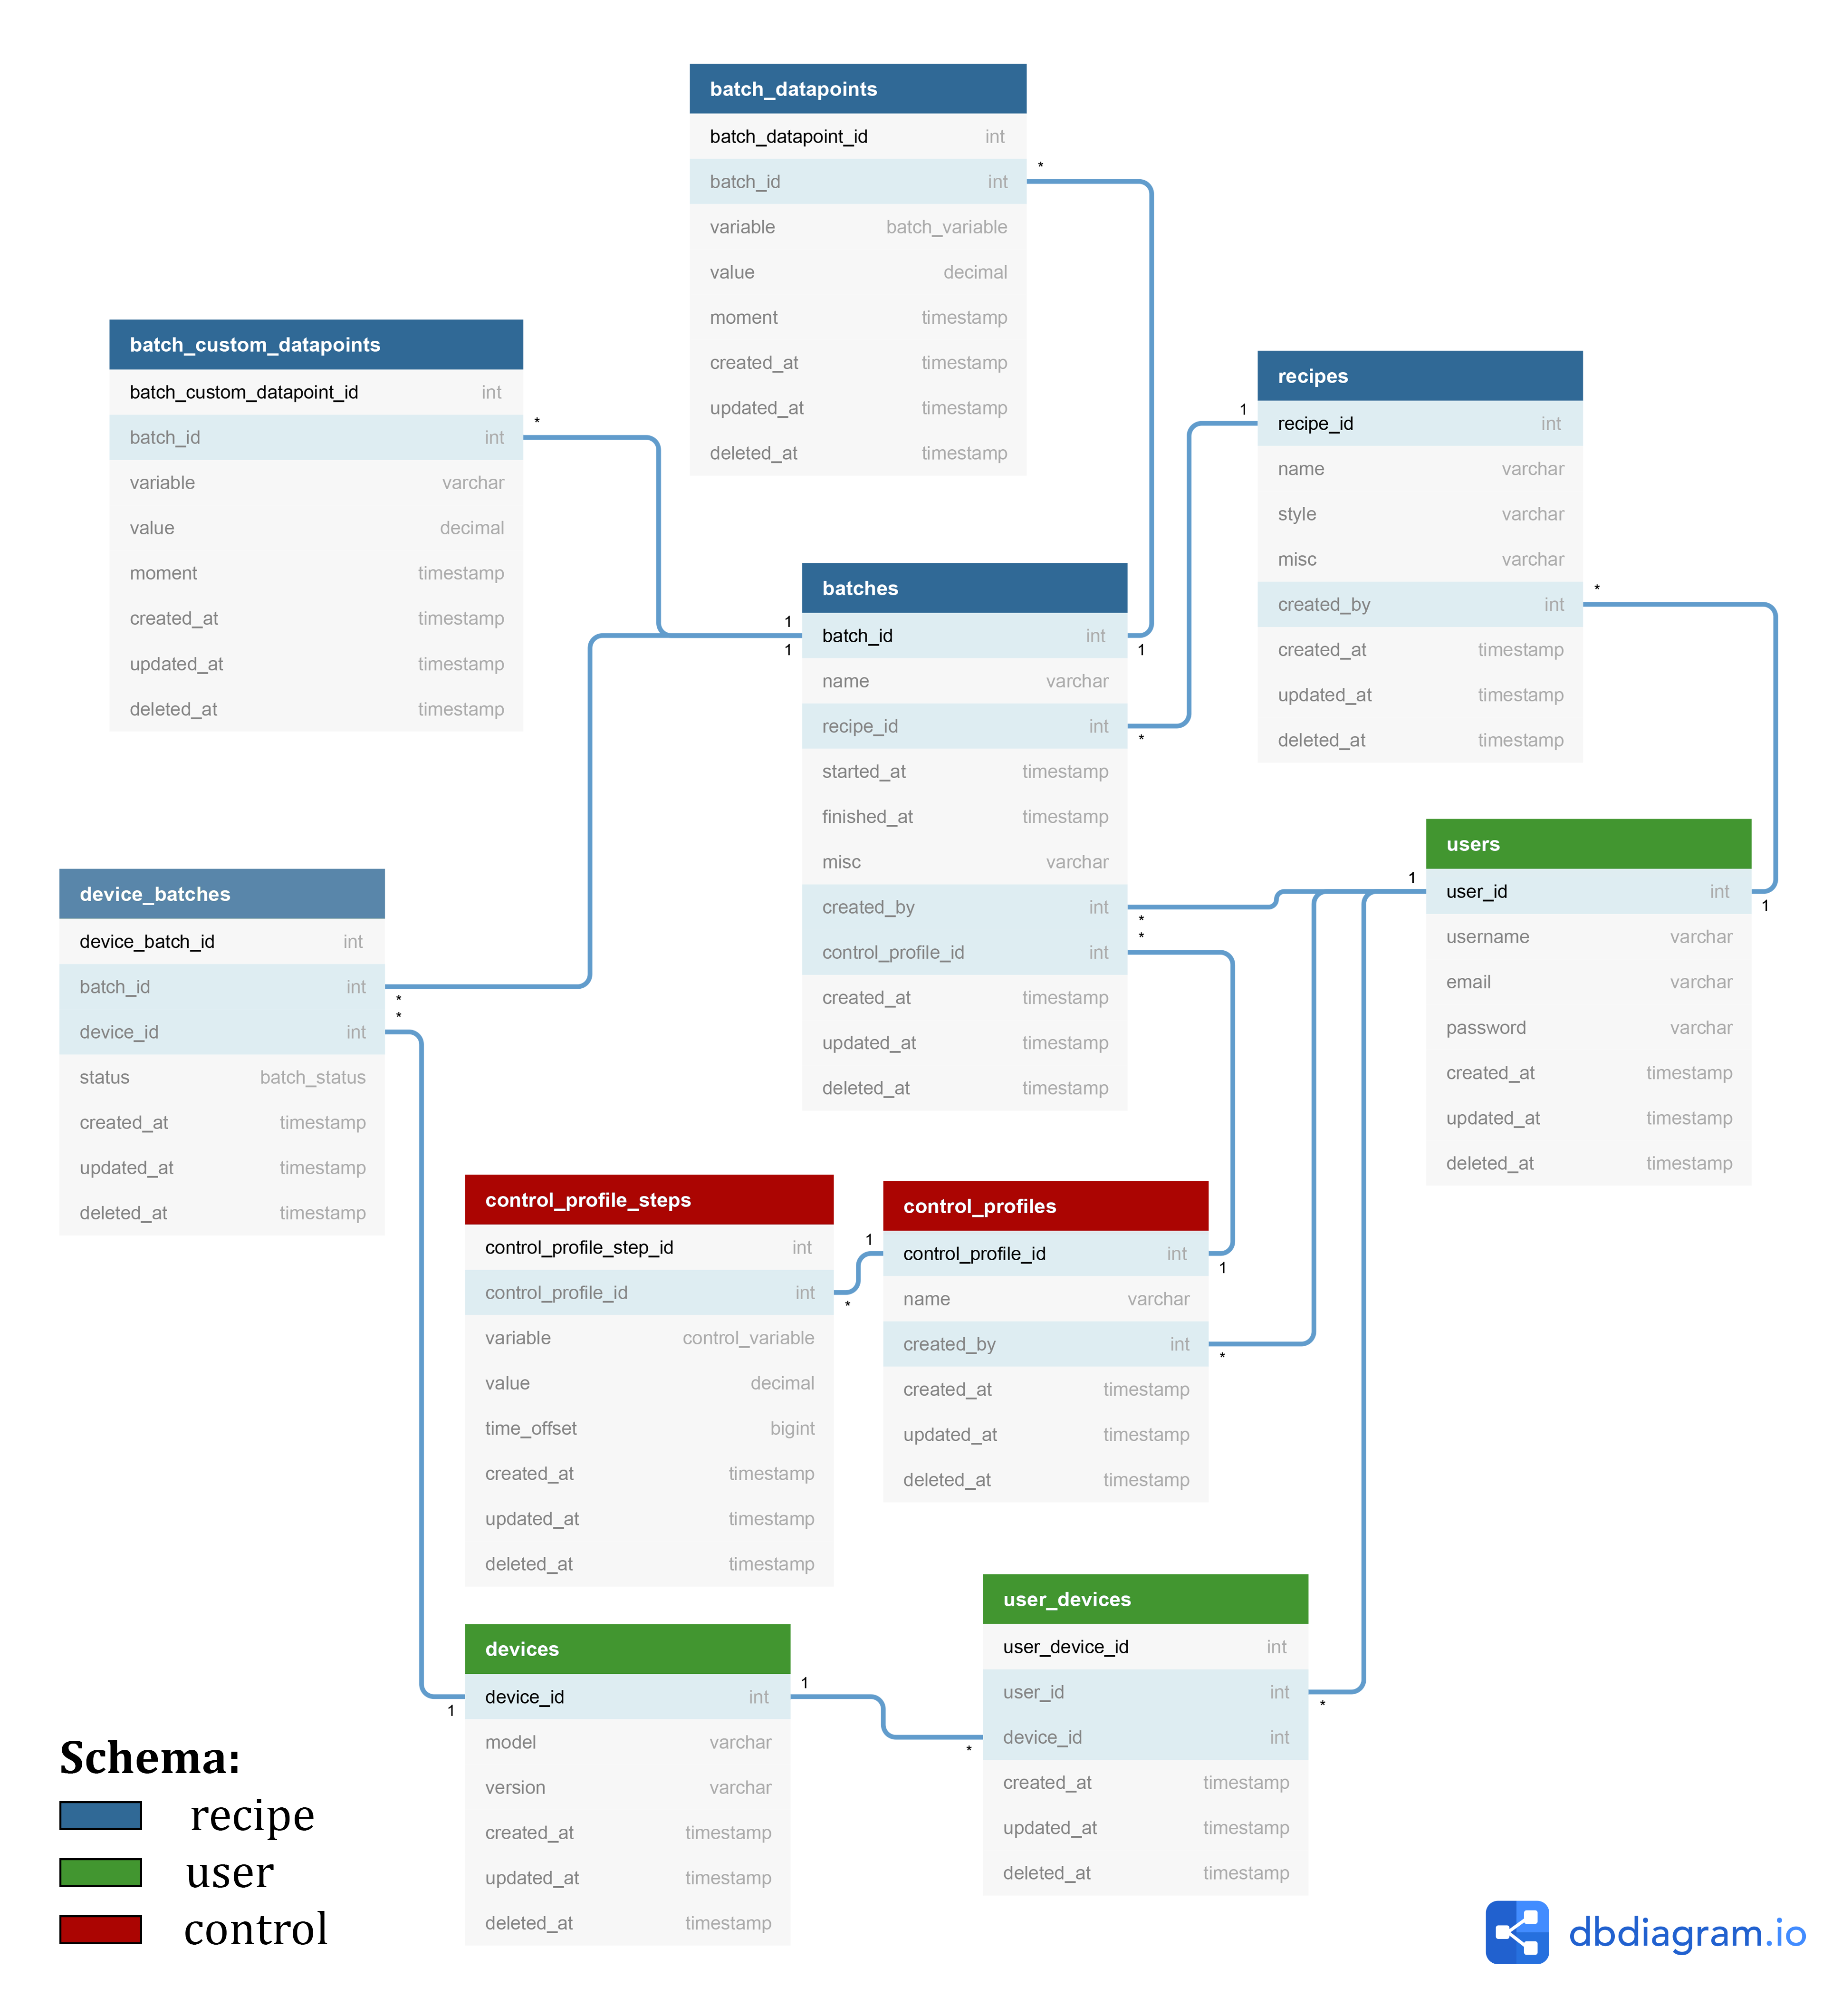
\includegraphics[scale=0.15]{figuras/projeto/software/banco_de_dados.png}
    \caption{Diagrama de Entidade-Relacionamento.}
    \label{fig:diagrama_entidade_relacionamento}
\end{figure}

\subsection{Arquitetura de Software}

A arquitetura de software do projeto foi estruturada tendo como base o fluxo da informação como especificado nos casos de uso e os conceitos de arquitetura de microsserviços. Dessa forma, foram definidas quatro camadas para organizar os sistemas a serem implementados: Camada de Interface, contemplando as interfaces utilizadas diretamente pelos atores; Camada Intermediária, contendo um API Gateway para isolar os microsserviços das interfaces e um message broker para intermediar a comunicação entre dispositivo e sistema; Camada de Negócio, contendo os microsserviços que exercem as regras de negócio do sistema; e Camada de Persistência, com os serviços de armazenamento de dados. Os componentes de cada camada são descritos em detalhes quanto a suas responsabilidades e detalhes de implementação em sequência. A arquitetura completa é representada visualmente pelo Diagrama de Componentes da figura \ref{fig:diagrama_componentes}.

%% TODO: Diagrama complexo em apêndice

\subsubsection{Camada de Interface}
A Camada de Interface contém os componentes que fornecem interface direta aos atores definidos na modelagem de casos de uso. Sua função, portanto, reside na interação com os atores e comunicação de suas ações para a próxima camada, a Camada Intermediária. São três componentes de interface que compõe essa camada: Aplicação Front-end, Aplicação Mobile e o Software Embarcado no dispositivo. 

A Aplicação Front-end é executada pelo navegador web do usuário do sistema, e permite que ele realize o cadastro e gerenciamento de todas as informações referentes ao sistema, como receitas, perfis de controle e lotes, ela também permite que o usuário visualize os dados gerados pelo dispositivo em formato de gráficos e tabelas. Essa aplicação contém o componente gráfico das telas que o usuário utilizará e algumas regras de validação simples, como campos obrigatórios de cadastro. As ações do usuário são traduzidas em requisições HTTP que são enviadas para o Serviço de API Gateway, na próxima camada. 

A Aplicação Mobile foi a solução encontrada para intermediar a comunicação entre usuário e dispositivo, suas principais funções são: enviar as informações necessárias para conexão à rede Wi-Fi do usuário, que é realizado pela tecnologia de bluetooth, e informar o sistema que aquele dispositivo foi ativado por determinado usuário. Após essa configuração, o usuário poderá associar um lote de uma receita para o dispositivo monitorar e controlar, e o dispositivo deve estar pronto para se comunicar com o sistema por meio de mensagens.

O Software Embarcado no dispositivo, além das funcionalidades de monitoramento e controle, que são detalhadas nas seções de Modelagem de Controle e Projeto de Hardware, deve ser capaz de se comunicar via tecnologia bluetooth com a Aplicação Mobile, e enviar e receber mensagens via protocolo MQTT com o Message Broker da Camada Intermediária. O dispositivo deve enviar mensagens com os dados que estão sendo coletados durante a fermentação, como temperatura, densidade relativa e pH, e receber informações sobre um novo lote que foi alocado para ele realizar o controle.

\subsubsection{Camada Intermediária}

Toda a comunicação entre os atores e o sistema é realizada por mediação da Camada Intermediária. O tráfego pode ocorrer pelos protocolos HTTP ou MQTT. O fluxo por HTTP é mediado pelo Serviço de API Gateway, que roteia as requisições externas para os devidos microsserviços, enquanto que o fluxo MQTT, composto por mensagens, é controlado pelo Message Broker, que organiza as mensagens nos fluxos dispositivo para sistema e sistema para dispositivo.

O Serviço de API Gateway funciona como um serviço de proxy reverso que, além centralizar as solicitações do usuário, consolida o resultado de cada microsserviço necessário para atender uma demanda. Apesar de ser um serviço muito simples, ele é importante por questões de segurança, uma vez que apenas um endereço fica exposto externamente e a autenticação externa é centralizada nele, e também por questões de escala futura, sendo mais fácil implantar um balanceador de carga ou sistema de fila de processamento com essa separação de serviços, caso seja necessário no futuro.

O Message Broker é simplesmente um corretor de mensagens, que opera sobre o protocolo MQTT, e é responsável pelo recebimento, entrega e armazenamento das mensagens que trafegam no sistema. O protocolo MQTT foi escolhido por ser extremamente leve e desenvolvido especialmente para o uso em Internet das Coisas.
    
\subsubsection{Camada de Negócio}
    
\subsubsection{Camada de Persistência}

\begin{figure}[ht]
    \centering
    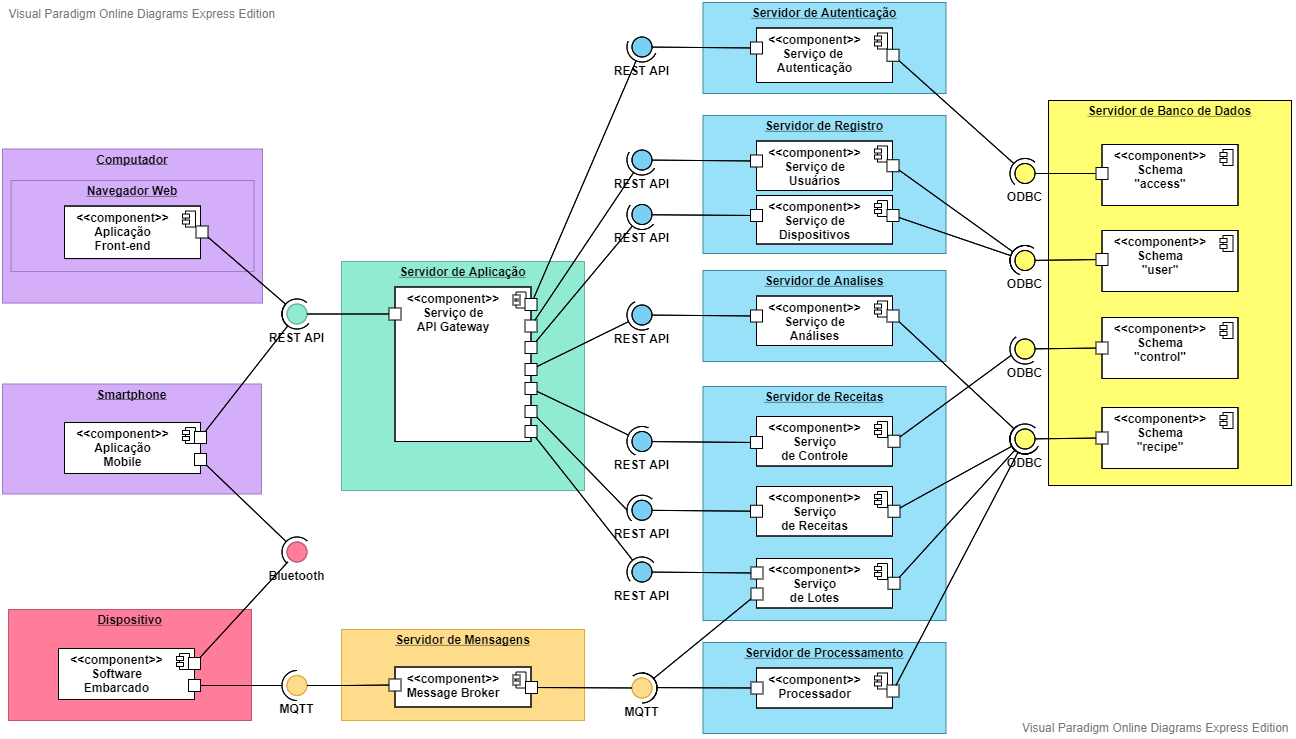
\includegraphics[scale=0.50, angle=270]{figuras/projeto/software/diagrama_componentes.png}
    \caption{Diagrama de Componentes.}
    \label{fig:diagrama_componentes}
\end{figure}

\subsection{Definição de Tecnologias}

\subsection{Projeto de Implantação}

\subsection{Protótipos das Interfaces}
%% TODO: Apêndices




\chapter{Implementação}

% // TODO: Escrever Implementação (Software e Hardware)
\section{Implementação de Hardware}

\subsection{Sensor de Temperatura}

O sensor de temperatura DS18b20 é alimentado pelos pinos de 5V e GND (terra) do microcontrolador. seu sinal de leitura é enviado para uma porta digital, sendo utilizado um resistor de 4,7 k$\Omega$ como pull up, caso exista uma leitura errada do sensor. A figura \ref{fig:micro_temp} ilustra a conexão do microcontrolador com o sensor de temperatura. 


\begin{figure}[h]
    \centering
    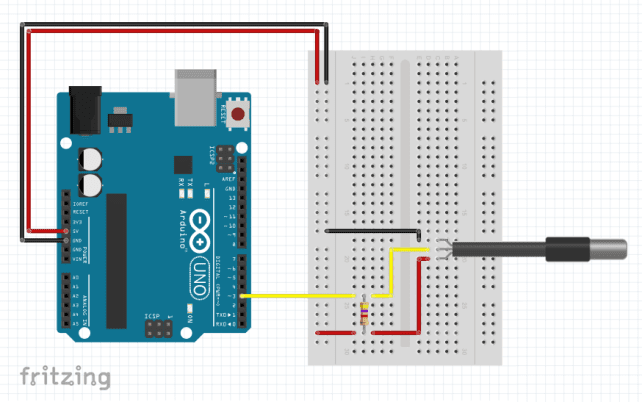
\includegraphics[scale=0.40]{figuras/implementacao/hardware/DSsensor.png}
    \captionsource{Esquema de conexão entre microcontrolador e sensor de temperatura DS18B20.}{https://portal.vidadesilicio.com.br/}
    \label{fig:micro_temp}
\end{figure}


O excerto de código em linguagem Arduino a seguir representa a função utilizada para ler o valor de saída do sensor. A biblioteca OneWire (\url{https://github.com/PaulStoffregen/OneWire}) implementa o protocolo proprietário de comunicação serial da Dallas Semicondutor, fabricante do sensor. Ela é utilizada em conjunto com a biblioteca livre DallasTemperature (\url{https://github.com/milesburton/Arduino-Temperature-Control-Library}) para estabelecer a comunicação com o DS18B20.

\begin{lstlisting}[language=C]

#include <OneWire.h>
#include <DallasTemperature.h>
#define ONE_WIRE_BUS D6

OneWire oneWire(ONE_WIRE_BUS);
DallasTemperature sensors(&oneWire)

void setup() {
    sensors.begin();
}

float readTemperature() {
    return sensors.getTempCByIndex(0);
}

\end{lstlisting}


\subsection{Sensor de pH}

O sensor de pH é conectado a um circuito auxiliar que trata o sinal proveniente da ponta de prova. Esse circuito é conectado aos pinos de 5V e GND do microcontrolador para alimentação, e envia do dado coletado por meio de sinal analógico, como observado na figura \ref{fig:micro_ph}. 


\begin{figure}[h]
    \centering
    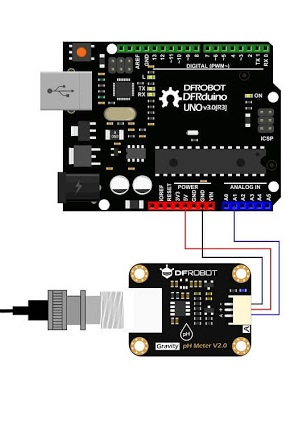
\includegraphics[scale=0.65]{figuras/implementacao/hardware/micro_ph.jpg}
    \caption{Esquema de conexão entre microcontrolador e sensor de pH E-201-C.}
    \label{fig:micro_ph}
\end{figure}


Para utilização desse sensor, é necessário sua calibração, que consiste na medição da tensão de saída do sensor em soluções com diferentes concentrações de \(H^+\) e obtenção de uma equação linear que traduza a voltagem medida em um valor de pH. Para isso utilizadas soluções tampão com pH iguais a 4, 7 e 10. A calibração seguiu o seguinte processo:
\begin{enumerate}
    \item Com a solução de pH igual a 7, ajustar o ganho do circuito (por um potenciômetro) até que a leitura de voltagem seja 2,5 Volts. Essa tensão foi escolhida de forma a coincidir valor médio da tensão de alimentação do circuito com o valor médio da escala de pH;
    \item Capturar a tensão medida nas soluções com pH 4 e 10;
    \item Aplicar regressão linear, minimizando a soma dos erros quadráticos, obtendo a reta que relaciona a tensão medida com o pH da solução
\end{enumerate}


Com os valores obtidos na tabela \ref{tab:calibra_ph}, foi obtida a equação linear \ref{eq:pH}.

\begin{equation}
    pH = 2.0171 \cdot Voltagem + 1.7152
    \label{eq:pH}
\end{equation}


\begin{table}[H]
    \begin{center}
        \begin{tabular}{ |c|c| } 
            \hline
            Voltagem & pH \\
            \hline
            2.50 & 7.0 \\ 
            \hline
            1.20 & 4.0 \\ 
            \hline
            4.16 & 10.0 \\ 
            \hline
        \end{tabular}
        \caption{\label{tab:calibra_ph}Medições de tensão em soluções tampão para calibração do sensor de pH.}
    \end{center}
\end{table}


A leitura do pH medido pelo sensor pelo microcontrolador segue o seguinte algoritmo:
\begin{enumerate}
    \item Valor inteiro entre 0 e 1024 recebido pelo sensor é lido na porta analógica;
    \item Valor lido é convertido em uma diferença de tensão seguindo \(Voltagem = medida \cdot 5 / 1024\);
    \item Diferença de tensão é convertida na leitura de pH seguindo equação linear obtida na calibração do sensor.
\end{enumerate}


% \begin{lstlisting}[language=C]

% int ph_pin = A0;

% float readPH() {
%     int measure = analogRead(ph_pin);
%     double voltage = measure * 5 / 1024;
%     return 2.0171 * voltage + 1.7152;
% }

% \end{lstlisting}

\subsection{Sensor de pressão diferencial para medida de densidade}

A medição de densidade foi implementada indiretamente através do sensor de pressão diferencial MP3V5010DP. Esse sensor será inserido no líquido fermentado através de dois tubos posicionados em uma distância fixa de 18 centímetros. A densidade será inferida através da fórmula: 

\begin{equation}
    \rho = \frac{\Delta P} {g \cdot \Delta h}
\end{equation}

O chip Pmod DPG1 se comunica com o microcontrolador através da interface periférica serial (SPI), que é um sistema de comunicação que utiliza as portas: SCK: Serial Clock (output from master), MISO: Master In Slave Out (data output from slave) e SS: Slave Select.

O sensor é alimentado com 3.3 V e é utilizado um conversor de nível lógico bidirecional para converter o sinal digital de 5V para a tensão do sensor. A biblioteca SPI (https://github.com/PaulStoffregen/SPI) foi utilizada para realizar essa comunicação e leitura. O valor recebido pelo microcontrolador é convertido através da fórmula fornecida no datasheet do chip:

\begin{equation}
    \Delta P = \frac{\frac{value/{4096} - 0.08}{0.08} 
\end{equation}

\subsection{Conexão e Comunicação do Microcontrolador}

Com os sensores propriamente conectados e calibrados, o microcontrolador foi configurado para se conectar à Internet através de conexão \textit{Wi-Fi} e a enviar os dados coletados por meio do protocolo MQTT. O Wemos D1 é controlada pelo módulo ESP8266, de forma que ofereça conectividade \textit{Wi-Fi} nativa. 
A biblioteca ESP8266\textit{Wi-Fi} (\url{https://github.com/esp8266/Arduino/tree/master/libraries/ESP8266WiFi}) foi utilizada para estabelecer a conexão \textit{Wi-Fi}, em conjunto com a biblioteca PubSubClient (\url{https://github.com/knolleary/pubsubclient}) para publicar mensagens e se inscrever em tópicos MQTT. 


% // TODO: Colocar código completo em Apêndice e discutir Fluxo completo aqui


\subsection{Controle de Temperatura}

Um controlador de malha fechada proporcional interativo derivativo (PID) é utilizado para controlar a temperatura do fermentador. Esse método é amplamente utilizado na indústria, possuindo boa precisão e confiabilidade, além de ser facilmente sintonizado. Inicialmente são definidos parâmetros analógicos e depois é criado o controle digital.


Sendo assim, o sistema com a pastilha de Peltier deve retirar do sistema uma quantidade de calor proporcional a essa recebida e gerada para manter uma temperatura estável abaixo do ambiente. Como a quantidade de calor retirada por um Peltier é proporcional a corrente, a tensão fornecida a pastilha é variada através de uma circuito ponte H que tem a sua amplitude de tensão de saída regulada por uma porta PWM.  

\subsubsection{Circuito Ponte H}

O circuito ponte H (figura \ref{fig:ponte_h}) permite que a amplitude e sentido da tensão de entrada da pastilha de Peltier seja controlado digitalmente por um sinal PWM (Pulse Width Modulation) do microcontrolador. No Software embarcado, um valor entre 0 e 255 é utilizado para definir o duty cycle da onda quadrada do sinal PWM, como exemplificado na figura \ref{fig:pwm}. 


\begin{figure}[H]
    \centering
    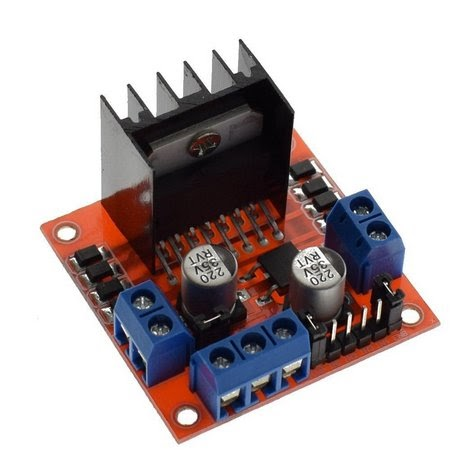
\includegraphics[scale=0.35]{figuras/implementacao/hardware/ponte_h.jpg}
    \captionsource{Modelo ponte H - L298N.}{https://mercadolivre.com.br/}
    \label{fig:ponte_h}
\end{figure}

\begin{figure}[H]
    \centering
    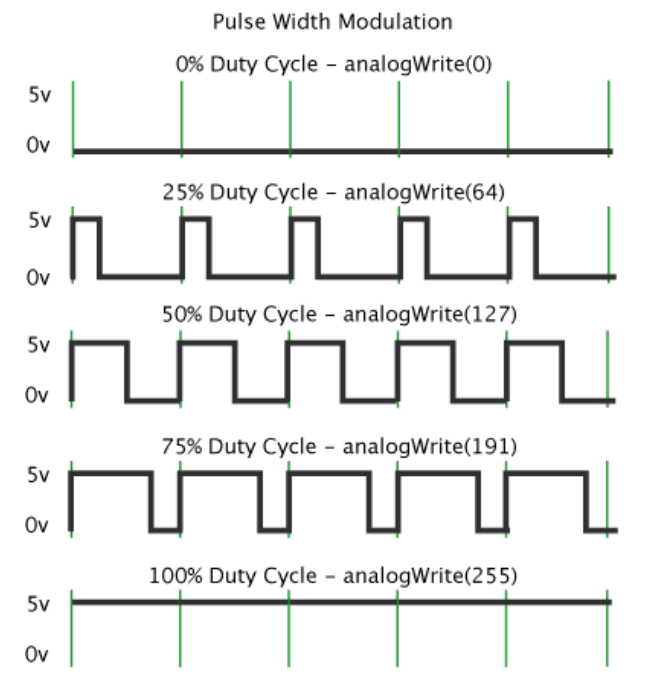
\includegraphics[scale=0.30]{figuras/implementacao/hardware/pwm.png}
    \captionsource{Onda quadrada do sinal PWM para alguns valores especificados no microcontrolador.}{https://www.arduino.cc/}
    \label{fig:pwm}
\end{figure}


\subsubsection{Montagem do Dispositivo}

Com as definições de controle discutidas, foi projetado o dispositivo da figura \ref{fig:dispositivo_term}, em escala aproximada. O dispositivo pode ser dividido em três partes descritas a seguir:

\begin{enumerate}
    \item Parte quente : Essa parte é ligada na face quente da pastilha e é formada por uma ventoinha e um dissipador de calor. Uma boa dissipação de calor garante uma melhor eficiência da partilha e permite que ela forneça quantidades de calor maiores para o sistema;
    \item Pastilha de Peltier: Pastilha que recebe a corrente e transforma energia elétrica em térmica. A face quente e face fria são isoladas por material isolante térmico, que ajuda na não interferência entre as partes e melhora a eficiência do sistema;
    \item Parte fria: essa parte é ligada na face fria da pastilha. Ela retira calor do sistema através de uma placa de cobra e barras de aço inox. Apesar do cobre ter uma condutividade térmica melhor, o aço inox foi escolhido para fazer a transmissão para o mosto + leveduras, por não interferir no seu gosto na exposição de pHs menores. 
\end{enumerate}


\begin{figure}[H]
    \centering
    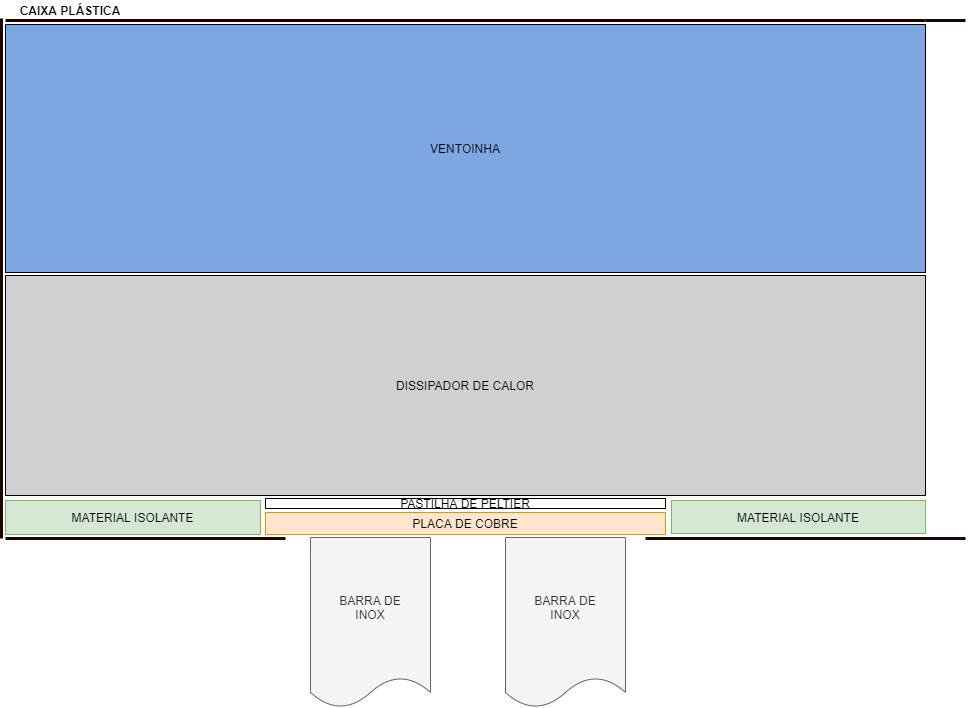
\includegraphics[scale=0.45]{figuras/implementacao/hardware/montagem.png}
    \captionsource{Esquema do perfil do dispositivo controlador de temperatura, escala aproximada.}{Autores}
    \label{fig:dispositivo_term}
\end{figure}



\chapter{Testes e Avaliação do Protótipo}

% // TODO: Escrever Testes e Avaliação do Protótipo
\textcolor{red}{\{Comentários sobre o funcionamento do protótipo completo, como foi testado e resultados obtidos\}}


\chapter{Considerações Finais}

\section{Conclusões do Projeto de Formatura}

\section{Contribuições}

\section{Perspectivas de Continuidade}


% TODO: Remover teste de referência
Testando referência bibliográfica como descrito em \cite{YeastWhite} e também em \cite{FermentationMunroe}.

% ========== Referências ==========
% --- IEEE ---
%	http://www.ctan.org/tex-archive/macros/latex/contrib/IEEEtran
%\bibliographystyle{IEEEbib}

% --- ABNT (requer ABNTeX 2) ---
%	http://www.ctan.org/tex-archive/macros/latex/contrib/abntex2
\bibliographystyle{abntex2-num}
\bibliography{./referencias/bibliografia} %Localização do arquivo bibliografia.bib
%\bibliography{}


% ========== Apêndices (opcional) ==========
\apendice{}
\chapter{Protótipos das Interfaces}

\label{appendice:prototipos}

% ========== Anexos (opcional) ==========
\anexo
\chapter{}



\end{document}
